\documentclass{iopjournal}
\usepackage{lmodern}
\usepackage{color}
\usepackage{xcolor}
\usepackage{amsmath}
% \usepackage{algorithmic}
\usepackage{amsmath,amssymb}
\usepackage{tikz-cd}
\usepackage{multicol}
\usepackage{algorithm}
\usepackage{algpseudocode}
\usepackage{amsfonts}
\usepackage{amsthm}
\usepackage{graphicx}
\usepackage{silence}
\usepackage{fancyhdr}
\usepackage{hyperref}
\usepackage[utf8]{inputenc}
\usepackage{textcomp}

\usepackage{lmodern}
% \WarningFilter{caption}{Unknown document class}
% \usepackage[compatibility=false]{caption}
\usepackage{subcaption}
\usepackage{float}
\usepackage{verbatim}
\usepackage{balance}
%\usepackage[utf8]{inputenc}

\hbadness=10000
\vbadness=10000
\hfuzz=2pt
\vfuzz=2pt

% \theoremstyle{thmstyleone}%
% \newtheorem{theorem}{Theorem}
% \newtheorem{proposition}[theorem]{Proposition}
\begin{document}
\articletype{Paper}

\title{Bio-inspired Robotic Fish Enabled Oil Spillage Monitoring}

\author{Muhammad Umar Masood$^1$\orcid{0000-0002-2500-2446}, Navid Khiabani$^2$, Kianoosh Karimi$^1$, Wenyu Zuo$^3$, Sarah Adaryan$^4$, Erin B. Porter$^4$, Haleh Ardebili$^1$, Rafael Verduzco$^4$ and Zheng Chen$^{1,*}$}

\affil{$^{1}$Department of Mechanical \& Aerospace Engineering, University of Houston, Houston, TX 77004, USA}

\affil{$^{2}$Materials Science and Engineering Program, University of Houston, Houston, TX 77004, USA}

\affil{$^{3}$University of Houston Energy Institute, Houston, TX, USA}

\affil{$^{4}$Department of Chemical and Biomolecular Engineering, Rice University, Houston, TX 77251, USA}

\affil{$^{*}$Author to whom any correspondence should be addressed.}

\email{zchen43@central.uh.edu}
%\thanks{Manuscript received April 19, 2005; revised August 26, 2015.}}
% \maketitle

% As a general rule, do not put math, special symbols or citations
% in the abstract or keywords.
\keywords{OECT, Robotic Fish, Bio-inspired, Oil Sensing}
\begin{abstract}
This paper introduces a fully integrated robotic sensing system for autonomous oil detection that combines an organic electrochemical transistor (OECT) sensor with a bio-inspired robotic fish platform. The OECT sensor is engineered to identify crude oil in water-based environments, including seawater, with high sensitivity and stability, while a robot-compatible signal conditioning circuit enables real-time detection and classification of oil during operation. The AquaNavigator robotic fish offers mobility, precise control, and modular payload capacity, enabling seamless integration of the sensing module without degrading its underwater performance. Laboratory experiments confirm that the OECT sensor can detect oil concentrations down to 10 µg, and the conditioning circuit facilitates effective onboard data collection. Tests conducted in an indoor water pool demonstrate that the integrated robotic platform can reliably detect oil spills while simultaneously performing pipeline tracking, thereby validating the practicality of a mobile bio-inspired system for locating sources of oil contamination in aquatic environments. The proposed system is well-suited for applications in environmental monitoring, underwater exploration, and search and rescue missions.
\end{abstract}
% Note that keywords are not normally used for peerreview papers.

\section{Introduction}
Until 2017, approximately 37\% of global crude oil production was carried out through offshore drilling \cite{energyocean}. While crude oil is highly valuable for energy generation, it is also a major contributor to marine pollution. Oil spills may result from accidents, equipment failures, leaks, or natural disasters. Such spills can cause severe harm to marine organisms \cite{Almeda2014}, entire ecosystems \cite{Soloneski2015}, and coastal populations \cite{Albers1982}. Consequently, the detection and continuous monitoring of oil spills are essential to reduce their impact and avoid additional damage. In general, oil leak detection methods are categorized into internal (software-based) and external (hardware-based) techniques. Internal methods rely on computational approaches, whereas external methods are usually grounded in local or remote sensing, and can be further divided into sensing/detection devices and visual or surveillance systems \cite{cramer2015}.

The most widely used internal techniques include mass–volume balance \cite{martins2010assessment}, negative pressure waves (NPW) \cite{hou2013pipeline}, pressure point analysis (PPA) \cite{bin2011pressure}, and dynamic modeling \cite{vitkovsky2007experimental}. These computational approaches rely on internal fluid measurement devices to track critical parameters along the pipeline \cite{ostapkowicz2016leak}. Differences between the measured values at the pipeline’s inlet and outlet are examined to identify and locate potential leaks. While internal methods are well suited for real-time surveillance and can accurately detect and pinpoint leaks, they typically entail substantial implementation costs and are sensitive to measurement noise, which can result in false alarms \cite{reda2024roadmap}.

External leak detection approaches are generally more economical than internal ones and provide greater precision in identifying the exact leak location. The first subgroup of such techniques uses sensors to observe the environment surrounding the pipeline, thereby enabling the recognition of irregularities and potential leak incidents \cite{ho2020inspection}. Irrespective of the underlying sensing mechanism, these methods usually require direct contact between the monitoring infrastructure and the sensing device, including acoustic \cite{martini2016leak}, fiber optic \cite{jacobsz2024performance}, fluorometric \cite{jasper2012oil}, and capacitive \cite{dario2019method} sensors. All of these sensors operate by detecting variations in the environmental or physical conditions around the pipeline to pinpoint leak locations. Nevertheless, depending on the specific use case, certain sensor types may be more practical or advantageous than others. For instance, acoustic and fiber optic sensors are commonly used for monitoring long subsea pipeline stretches because of their high sensitivity and performance, yet their installation and operation can be expensive and technically demanding. In contrast, capacitive and fluorescence-based technologies are relatively low-cost and perform well in controlled settings, but they generally exhibit lower reliability in harsh subsea environments \cite{adegboye2019recent}.

The second subcategory of external techniques is based on visual observation using optical cameras and video sensors. Under favorable visibility conditions, these systems can provide broad coverage and reliably detect leaks with a low false alarm rate; however, operational and logistical constraints limit their suitability for continuous, real-time monitoring. Recent developments in remotely operated vehicles (ROVs)\cite{hu2022underwater} have significantly enhanced the monitoring of offshore oil transport infrastructure, and the subsequent transition to autonomous underwater vehicles (AUVs)\cite{shukla2016application} has enabled more independent and efficient operations. Aerial and satellite imagery are also included in this group, serving as powerful tools for identifying large-scale oil spills; nonetheless, as previously discussed, their response time typically lags the actual moment the leak occurs. Taking into account the advantages and drawbacks of each method, the most effective subsea pipeline leak detection strategies appear to be those that integrate direct sensing technologies with inspections carried out by ROVs and AUVs\cite{lukonge2020leak}.

Deploying sensors on robotic platforms is standard practice, particularly in settings where human presence is unsafe or impractical. This applies not only to underwater environments but also to terrestrial robots and aerial drones \cite{Yu2019}. In the underwater domain, remotely operated vehicles (ROVs) are the predominant platforms, widely used for inspecting and monitoring submerged infrastructure. Qasem et al. \cite{Qasem2019} introduced a multisensor ROV system capable of detecting oil spills through camera-based surveillance combined with image processing methods. Yao et al. \cite{Yao2024} proposed an ROV-mounted thin oil slick detection system that estimates the time-of-flight of ultrasonic signals using a generalized sparse iterative covariance estimation (SPICE) approach. Other ROV-based solutions for oil spill detection exploit acoustic and optical imaging techniques \cite{Pocwiardowski2021,Du2025}. However, to the best of our knowledge, no robotic systems have yet been developed that rely on chemical sensors for oil spill detection.

However, such ROVs are typically costly, demand specialized operator training, and involve high system and operational expenses. In addition, the propulsion mechanisms they use inherently generate substantial water turbulence~\cite{Capocci2017}. In contrast, bio-inspired robotic fish are gaining attention in this field because they can swim smoothly and cause minimal disturbance to the aquatic environment \cite{Marras2012, Polverino2013}. These robots replicate the swimming kinematics of real fish, enabling them to traverse water with reduced drag and turbulence. As a result, they are well suited for tasks such as underwater inspection, monitoring, and exploration. In this work, we introduce a bio-inspired robotic fish platform capable of carrying an OECT sensor for oil spill detection. The platform follows a modular design, which facilitates straightforward integration of diverse sensors and payloads. This modularity allows the robotic fish to be tailored to multiple use cases, including environmental monitoring, underwater exploration, and search-and-rescue missions. Furthermore, the proposed platform is engineered to be cost-effective and user-friendly, broadening its accessibility to a diverse range of operators.

The rest of the paper is structured as follows. Section II details the OECT sensor along with the design of its signal conditioning circuit. Section III outlines the development and fabrication of the AquaNavigator robotic fish platform. Section IV covers the laboratory testing and validation of the signal conditioning circuit. Section V reports the experimental results obtained with the OECT sensor and the AquaNavigator platform in the water pool facility. Finally, Section VI summarizes the work and highlights directions for future research.

\section{OECT Sensor for Oil Detection}
The oil-sensing element employed in this study is an organic electrochemical transistor (OECT) previously introduced in \cite{porter2024detection}. This thin-film sensor consists of a PEDOT:PSS channel overlaid with a hydrophobic polystyrene coating, which facilitates the selective adsorption of crude oil. Upon contact with oil, the surface experiences a change in ionic permeability, leading to an increase in impedance and a corresponding decrease in source–drain current. The device functions reliably in aqueous media, including seawater, and can detect oil at concentrations down to 10 µg. It remains stable during long-term immersion and is compatible with fabrication on flexible substrates. Collectively, these characteristics render it well-suited for integration into mobile robotic platforms for in-situ environmental monitoring. This type of chemical sensor offers a broad range of potential applications \cite{adaryan2025organic}.

\subsection{OECT Sensor Fabrication}
Organic electrochemical transistors (OECTs) were fabricated on 2.5 cm $\times$ 1.0 cm glass substrates. Kapton tape was first applied to define the electrode geometry, after which 5 nm of titanium and 50 nm of gold were deposited by sputtering. Following electrode masking with Kapton tape, the channel region was spin-coated with a PEDOT:PSS formulation containing (3-glycidyloxypropyl)trimethoxysilane (1 wt\%), ethylene glycol (5 vol\%), and 4-dodecylbenzenesulfonic acid (0.25 vol\%) at 1000 rpm for 30 s, and then annealed at 140~$^\circ$C for 1 h. The channel was subsequently defined by mechanically etching the metal layers with a syringe needle, then overcoated with PEDOT:PSS and a further polystyrene (PS) layer. The hydrophobic PS layer facilitated oil adsorption upon contact, which altered the ionic permeability of the channel and, in turn, modulated the source–drain current of the OECT \cite{porter2024detection}. The main fabrication steps of the OECT sensor are summarized in Fig.~\ref{fig:OECT-fab-process}.
\begin{figure}
    \centering
    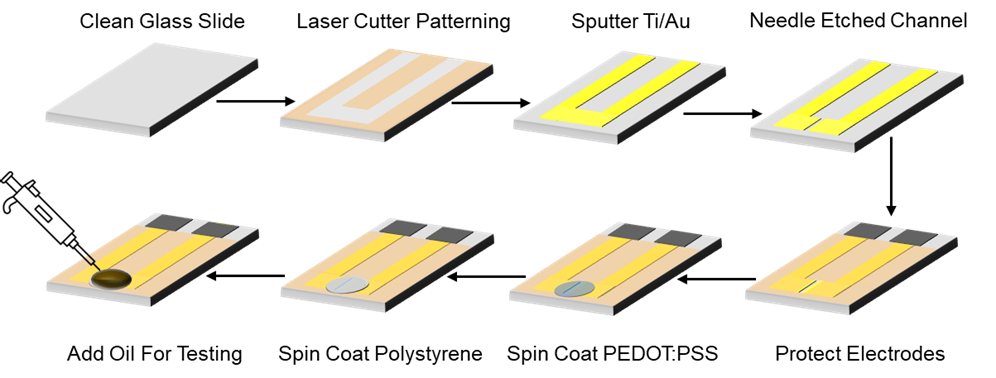
\includegraphics[width=0.75\textwidth]{figures/OECT-fab.png}
    \caption{OECT sensor for oil detection. The sensor is fabricated on a glass substrate with gold electrodes and a PEDOT:PSS channel coated with a hydrophobic polystyrene layer.}
    \label{fig:OECT-fab-process}  
\end{figure}

\noindent
\begin{figure}
    \centering
    \begin{minipage}[t]{0.3\linewidth}
    \centering
    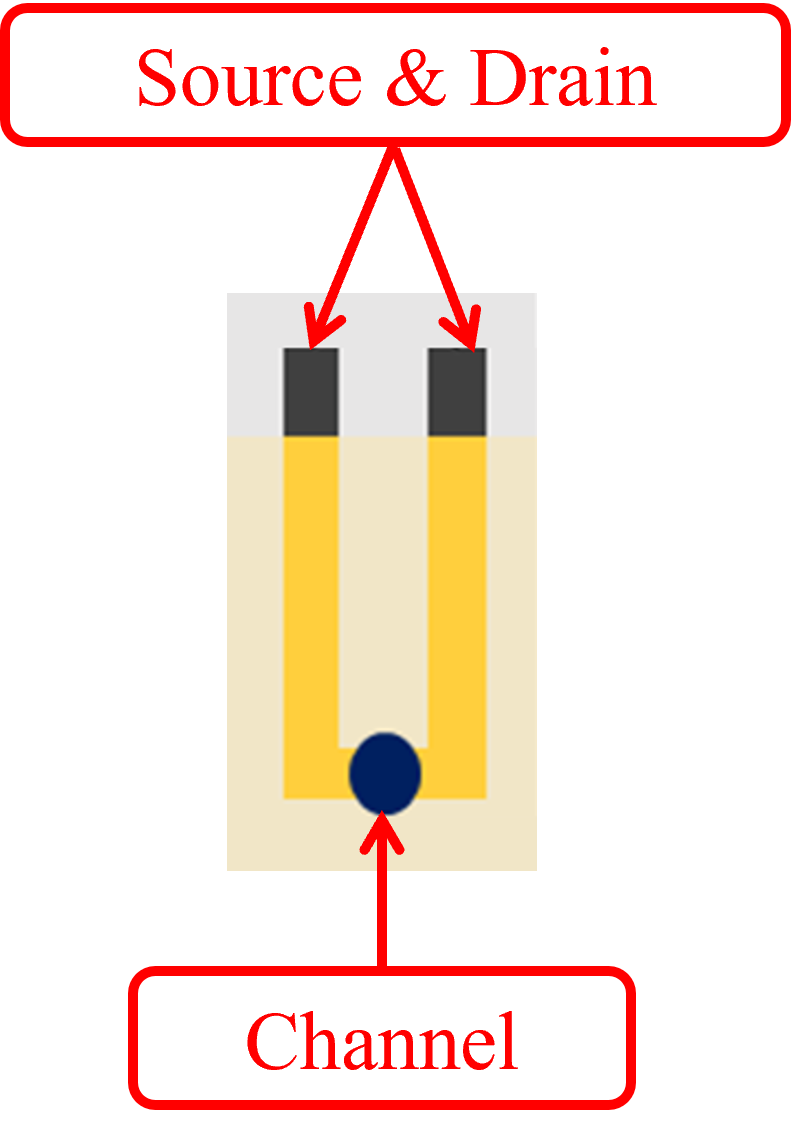
\includegraphics[width=\linewidth]{figures/oect-diagram.png}
    
    \textbf{(a)} OECT sensor schematic
    \end{minipage}
    \hfill
    \begin{minipage}[t]{0.45\linewidth}
    \centering
    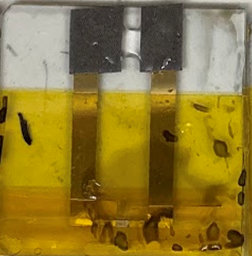
\includegraphics[width=\linewidth]{figures/oect-fabricated.png}

    \textbf{(b)} OECT sensor fabricated on glass substrate
    \end{minipage}
    \caption{OECT sensor: schematic and fabricated version}
    \label{fig:oect-scheme-fab}
\end{figure}

The OECT schematic and the fabricated glass-substrate device are shown in Fig.~\ref{fig:oect-scheme-fab}.

The transfer characteristics of the OECT were measured using a source meter. Additional electrochemical analyses were carried out to monitor variations in resistance and ionic permeability by means of cyclic voltammetry (CV) and electrochemical impedance spectroscopy (EIS). Fluorescence microscopy was employed to visualize the adsorption of crude oil on the coated surfaces. Contact angle measurements were performed to evaluate how the oil interacted with the sensing surface. In a previous study, this approach demonstrated improved oil spreading on coated samples compared to uncoated ones \cite{porter2024detection}.

\subsection{Lab Testing of the Sensor for Classification}
Using an OECT for crude oil detection offers several benefits: it is inexpensive to fabricate and remains stable in aqueous solutions. In addition, its transistor-like configuration enables straightforward signal amplification and readout. Together, these features support fast detection and straightforward deployment when the devices are integrated into robotic systems.  
From the OECT characterization, a gate voltage window of $-0.6$~V to $+0.6$~V is chosen to yield a detectable current while minimizing water electrolysis. At the same time, a constant source--drain bias of $-0.6$~V is applied. Measurements in pure water serve as the reference condition. The transfer characteristics of each OECT sensor are then obtained by recording the drain current as a function of gate voltage before and after introducing crude oil.

In previous research \cite{porter2024detection}, laboratory experiments showed that introducing oil into the system can impede electron transfer through the channel, thereby increasing both impedance and resistance. Consequently, the current in the transfer characteristics is reduced. Those laboratory measurements were conducted using cyclic voltammetry, which applies a linearly varying potential to the electrode in both forward and reverse directions. In the present study, a sawtooth gate voltage was used to acquire data for plotting current as a function of potential. A source measurement unit (SMU) was employed to track the current between the source and drain while holding the voltage constant. The laboratory equipment consisted of a Keithley 2100 Digital Multimeter for controlling and measuring the gate voltage, and a Keithley Series 2400 Source Measurement Unit for applying the drain–source voltage and measuring the corresponding current. The laboratory testing setup used for OECT sensor characterization is shown in Fig.~\ref{fig:oect-lab-testing}.
\begin{figure}
    \centering
    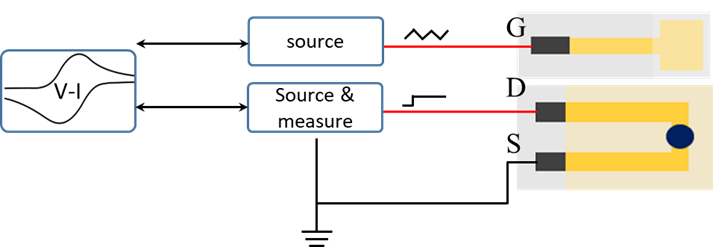
\includegraphics[width=0.65\textwidth]{figures/oect-smu-scheme.png}
    \caption{Schematic of the lab testing setup for OECT sensor characterization.}
    \label{fig:oect-lab-testing}
\end{figure}

\subsection{Signal Conditioning and Circuit Design}
While the laboratory configuration enabled accurate characterization of the sensor’s response to oil, it was impractical for real-time or mobile use. The source meter is bulky and consumes significant power, making it unsuitable for integration into autonomous platforms such as robotic fish. To address this limitation, a compact, dedicated signal-conditioning circuit had to be designed. This circuit needed to reproduce the waveform generation of the lab system—such as supplying sawtooth or square-wave voltages—while concurrently measuring very small currents with high resolution. The final design incorporated three primary channels: a variable gate-voltage output, a fixed drain-voltage supply, and a current-sensing input at the source. Proper signal conditioning enables clean capture of the sensor output, allowing subsequent classification algorithms to reliably identify the presence of oil during robotic missions in real-world environments.

To achieve this, a dedicated circuit is required that can replicate the main functions originally handled by the SMUs, including on-board data acquisition, while being compact and lightweight enough to mount on a small robot. The key roles of this circuit are to (1) provide a constant voltage to the source terminal of the OECT channel, (2) apply a gate voltage ranging from +0.6 V to -0.6 V, (3) measure the current flowing between source and drain, (4) enable data communication with the robotic fish, and (5) interface with the host computer via a UART connection. 
Current sensing is implemented using the Texas Instruments INA219, which, when paired with a $110\Omega$ shunt resistor, offers a current resolution of up to $10 \mu A$. Each voltage supply is generated using an MCP4725 digital-to-analog converter from Microchip Technology, which receives control signals from the main microcontroller over the Inter-Integrated Circuit (I2C) bus. The central controller for the entire system is the ESP32-C3 microcontroller from Espressif Systems. 
A block diagram summarizing the circuit’s operation is presented in Fig.~\ref{fig:CircuitBirdsEye}. Further circuit details and the complete schematic are included in the Supplementary Information section.
\begin{figure}[htbp]
    \centering
    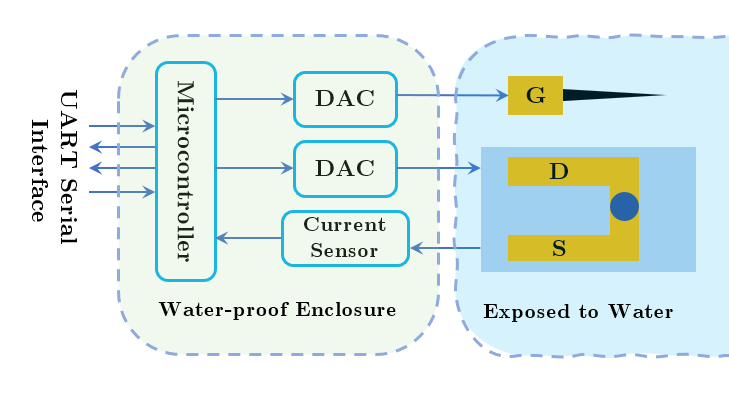
\includegraphics[width=0.75\textwidth]{figures/OECT-circuit-scheme.png}
    \caption{Block diagram of the OECT signal conditioning circuit.}
    \label{fig:CircuitBirdsEye}
\end{figure}

\subsection{Enclosure and Hardware}
To enable the use of this circuit on an underwater robot, a waterproof housing is also developed. The housing forms a sealed chamber with two watertight cable ports—one dedicated to power and data transmission, and the other accommodating the gate. The circuit is mounted at the bottom of this chamber. In the middle section of the housing, there is a cap equipped with an O-ring that ensures the enclosure is sealed. This cap also provides a channel for the cable and integrates an anode for the drain–source pair. The sensor must be installed facing downward at the cap so that its drain–source terminals make contact with the anode and cathode. Around the sensor, an extra sealing layer made of silicone rubber is added. A sealing cap is then placed over this layer and tightened, compressing the seal and preventing any water from reaching the sensor. All parts of the enclosure, including the caps, are fastened together with screws.


\section{AquaNavigator - Intelligent Robotic Fish}
To achieve autonomous, mobile oil spill monitoring, we incorporated the OECT sensing system into a custom-built robotic fish platform, termed the AquaNavigator. This submersible vehicle is engineered to function under both stationary and dynamic operating conditions, enabling patrols in confined tanks as well as along pipelines in open-water settings. The AquaNavigator acts as the physical host for the sensing circuitry, supplying power, locomotion, and data acquisition functionalities. Its streamlined, hydrodynamic body, propulsion components, and integrated electronics are optimized for stable underwater performance while reducing potential interference with the sensors. By embedding the oil detection system into this mobile platform, we aim to transition OECT sensors from controlled, laboratory-based experiments to deployment in realistic aquatic environments. The subsequent subsections detail the mechanical architecture, fabrication steps, waterproofing approach, and the incorporation of the sensing and control units.

\subsection{Design of AquaNavigator}
AquaNavigator is a robotic fish previously developed in \cite{masood2025visual}, with a focus on efficiency enabled by its double slider-crank (DSC) propulsion mechanism \cite{Zuo2021}. The robotic fish incorporates a buoyancy-based depth control (BCD) system \cite{Masood2023}, which provides an additional degree of freedom in depth, resulting in three degrees of freedom overall. The overall design and geometry of AquaNavigator are shown in Fig.~\ref{fig:design}. Its primary components are the tail assembly, the BCD and electronics enclosure, and the top cosmetic cover. 

The tail assembly integrates the DSC mechanism driven by a DC motor, along with a servo motor that sets the tail bias rotation angle. All elements in the tail assembly are rendered water resistant by applying epoxy resin at the component level. The BCD and electronics enclosure accommodates the control electronics, battery, and camera. This enclosure is sealed against water ingress using a face seal on its flanged interface. The top cosmetic cover is shaped to provide a streamlined, hydrodynamic profile and an aesthetically refined appearance. All structural components are manufactured using FormLabs\texttrademark{} Stereolithography (SLA) 3D printers.

The robotic fish is powered by a three-cell Lithium Polymer (LiPo) battery rated at 11.1 V and 1500 mAh, enabling continuous operation for approximately 60 minutes in a water tank environment. The main control board is based on a 32-bit ESP-32-C3 microcontroller, complemented by motor driver ICs. This on-board microcontroller executes all low-level control tasks and interfaces with a host computer via either wireless communication or a wired serial connection, selected according to the application requirements.
\begin{figure}[ht]
    \centering
    \begin{subfigure}[b]{0.6\textwidth}
        \centering
        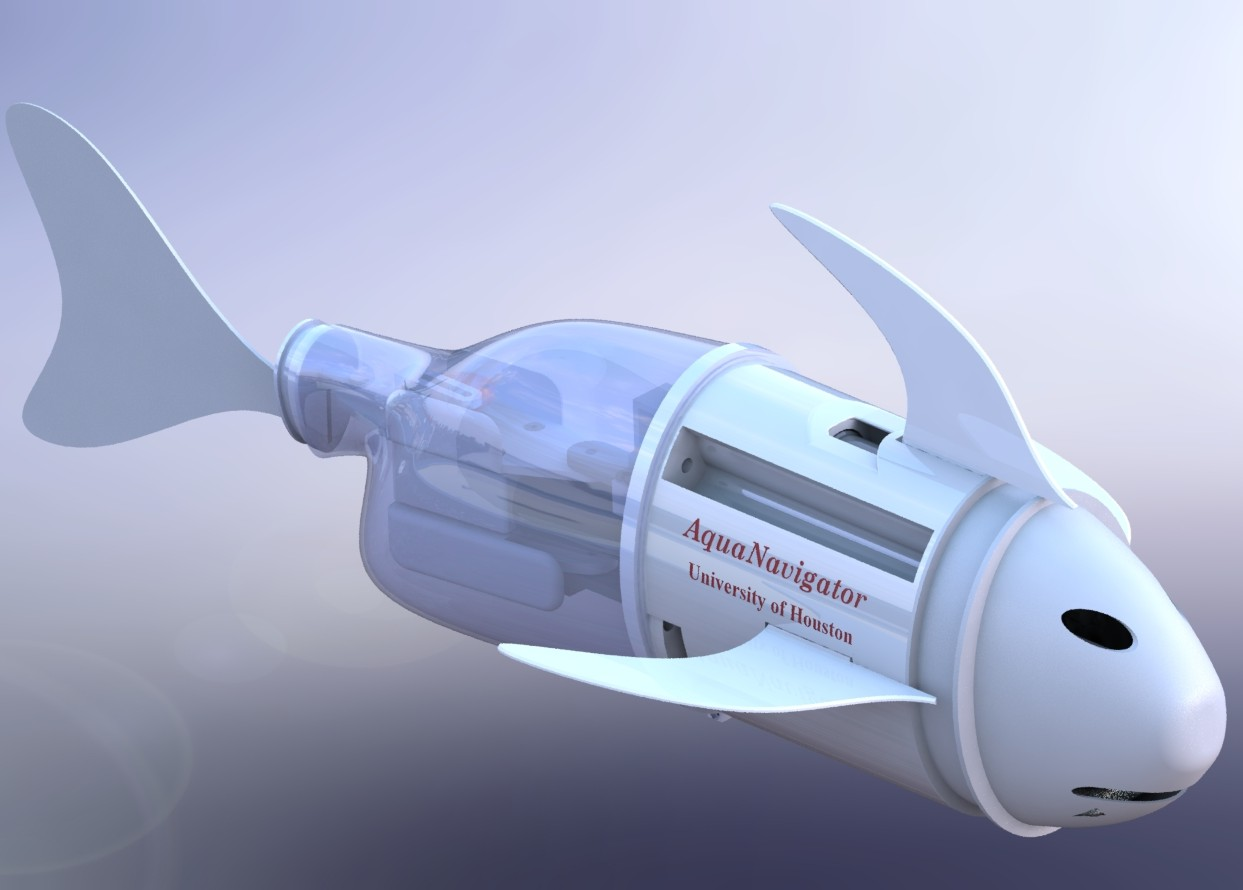
\includegraphics[width=\textwidth]{figures/Fish_v3_Solid.JPG}
        \caption{CAD design of the AquaNavigator}
    \end{subfigure}
    \hfill
    \begin{subfigure}[b]{0.9\textwidth}
        \centering
        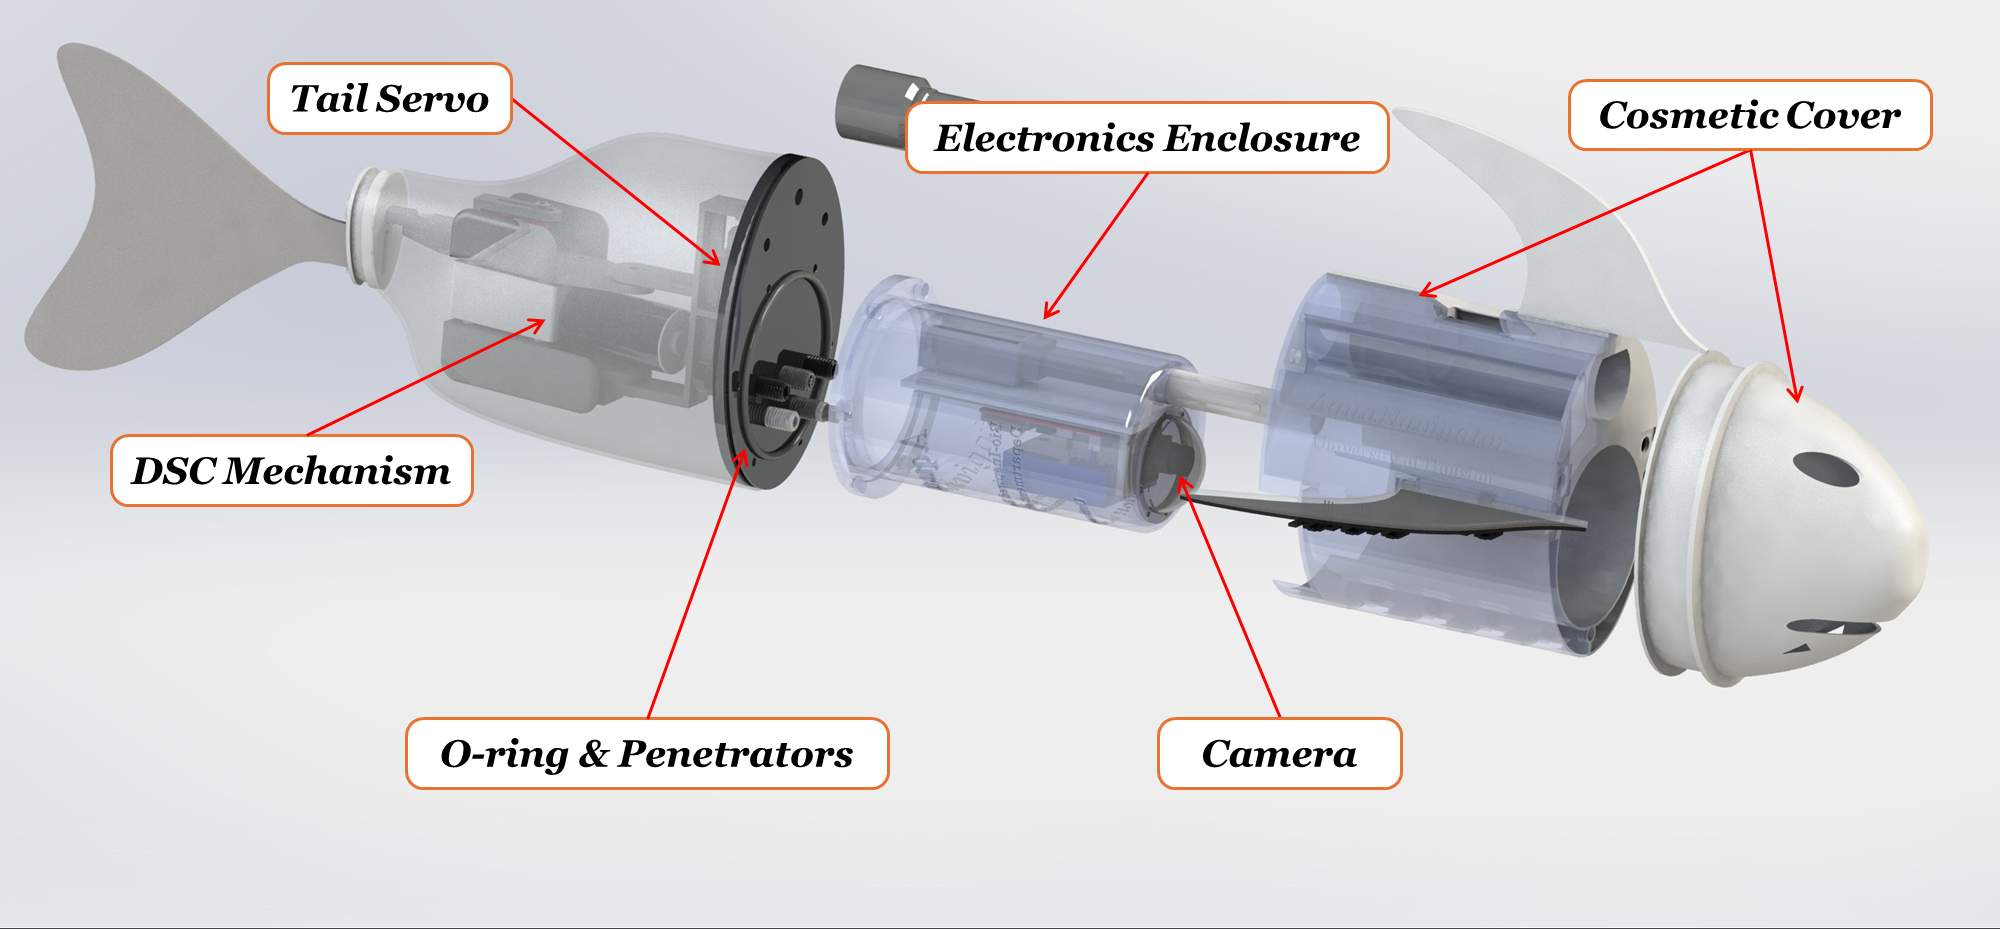
\includegraphics[width=\textwidth]{figures/Fish-Desgin-exploded.png}
        \caption{Exploded view showing main components}
    \end{subfigure}
    \caption{Design of AquaNavigator robotic fish platform.}
    \label{fig:design}
\end{figure}

\subsection{Modular Design}
A key design principle of the AquaNavigator is its modular architecture. The system incorporates a dedicated sensor enclosure and standardized electrical interfaces (UART, SPI, and I2C) on the main control board, enabling the integration of various sensor payloads without altering the robot’s physical structure. This modular approach has previously been validated for camera-based visual servoing \cite{masood2025visual} and is equally suitable for the chemical sensing payload described in this work.

For oil spill detection, where the OECT sensor is positioned on the robot’s body is a key design choice governed by how crude oil behaves in aquatic environments. Crude oil is hydrophobic and does not mix with water, and its density (typically 0.80–0.90 g/cm\textsuperscript{3}) is lower than that of both freshwater ($\approx$1.00 g/cm\textsuperscript{3}) and seawater ($\approx$1.025 g/cm\textsuperscript{3}). Consequently, spilled oil tends to rise and accumulate at the air–water boundary, forming a surface slick instead of dispersing evenly throughout the water column. This behavior persists even when leaks occur underwater: oil escaping from a submerged pipeline will move upward and pool near the surface. Therefore, at any given monitoring point, the maximum oil concentration is consistently located at or close to the water surface, so mounting the sensor on the top of the robot is the most effective way to maximize the likelihood of contact between the sensor transducer and the oil.

However, mounting a sensor package on top of the robot introduces a significant mechanical challenge in terms of stability. The static stability of an underwater vehicle depends on the relative locations of its center of gravity (CG) and center of buoyancy (CB): raising the CG above the CB diminishes the righting moment and can cause the platform to pitch or roll. Consequently, adding mass to the dorsal side of the fish risks disturbing the vehicle’s nominal trim.
To address this issue, several design strategies were implemented. First, the OECT sensor was housed in an enclosure fabricated via SLA 3D printing, incorporating a custom PCB. In contrast to metallic or otherwise dense housings, the SLA-printed enclosure is positively buoyant, which helps counterbalance the destabilizing influence of the added top mass by providing an upward force that supports the platform’s inherent buoyancy profile. Second, the sensor module was aligned with the fish’s longitudinal centerline to prevent the generation of an asymmetric rolling moment. Third, the AquaNavigator’s integrated buoyancy control system \cite{Masood2023} offers active regulation of depth and trim, allowing the vehicle to compensate for small alterations in the CG–CB relationship introduced by the top-mounted payload. Collectively, these measures preserve the hydrodynamic stability of the platform while enabling a top-mounted OECT sensor configuration that maximizes oil detection performance.

\subsection{Communication and GUI on Host Computer}
The AquaNavigator is capable of wireless communication (in shallow water only) and wired communication with the host computer. In different applications, the communication can be used to send the sensor data to the host computer for further processing, or to control the robotic fish. For the purpose of this study, to show the proof of concept, the robotic fish is tasked with tracking an oil pipeline in the water tank. The robotic fish has an onboard RGB camera, which can be used to track the pipeline using the Visual Servoing technique \cite{masood2025visual}. For this application, most of the computation is performed on the host computer running a Windows program developed in Python. The host computer is connected to the robotic fish using a USB cable, which provides a reliable and fast communication link. The program performs all the necessary computations, including, but not limited to; (1) image acquisition, (2) image processing, and hough transform to detect the pipeline, (3) control signal generation based on the visual servoing algorithm, (4) communicating the control signal to the robotic fish, and (5) showing the real-time video feed and control signals on the GUI. The GUI contains user controls to control the robotic fish in the manual operation mode, or set the parameters for the visual servoing algorithm in the autonomous operation mode. The GUI also displays the real-time video feed from the on-board camera, which can be used to monitor the operation of the robotic fish. The camera view is shown in Fig. \ref{fig:gui}.
\begin{figure}[t]
    \centering
    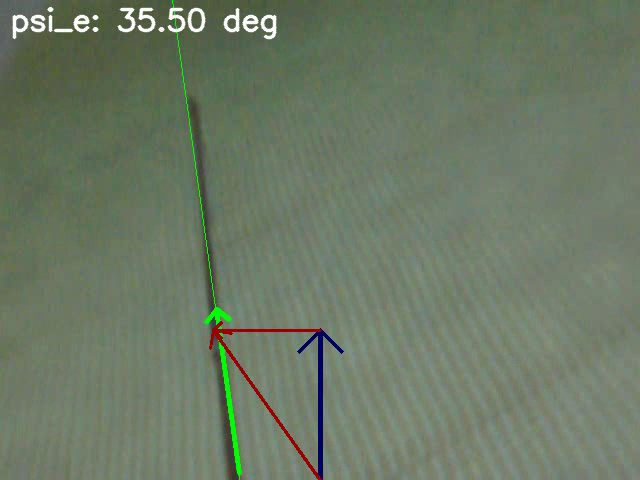
\includegraphics[width=0.6\textwidth]{figures/FishCamView.png}
    \caption{View as seen on the Graphical User Interface from the camera mounted on the robotic fish. The calculated $\psi_e$ angle is also overlaid on the frame.}
    \label{fig:gui}
\end{figure}

\subsection{Real-Time Classification of Oil Detection}

To enable on-the-fly detection of oil contamination during robotic operation, a pulse-amplitude-based classification routine is implemented and executed in real time on the host computer. The algorithm exploits the square-wave gate excitation already applied to the OECT: in clean water, the transistor responds to each gate pulse with a well-defined current amplitude, whereas the presence of oil in the channel reduces that amplitude due to the decrease in ionic permeability caused by oil adsorption. Rather than evaluating individual current samples, the method averages the pulse-response amplitudes over $N$ consecutive gate pulses, computing a normalized attenuation score $S$ that quantifies the relative drop in drain–source current with respect to a clean-water baseline amplitude $A_0$. When $S$ exceeds a preset detection threshold $\gamma$, the system raises an oil-detection flag. The complete procedure is formalized in Algorithm~\ref{alg:oil_detection}.

\begin{algorithm}[t]
\caption{Pulse-amplitude-based oil detection from OECT drain-source current}
\label{alg:oil_detection}
\begin{algorithmic}[1]
\Require Measured drain-source current $I_{DS}(t)$, input pulse timing, clean-water baseline amplitude $A_0$, detection threshold $\gamma$, number of pulses $N$
\Ensure Binary oil-detection decision $D \in \{\text{Oil}, \text{No Oil}\}$

\State Segment $I_{DS}(t)$ into $N$ pulse-response windows using the known square-pulse timing

\For{$k = 1$ to $N$}
    \State Select a pre-pulse interval in the $k$th window
    \State Select a post-pulse steady-response interval in the $k$th window

    \State Compute the low-state current
    \Statex
    \[
        I_{\mathrm{low},k}
        =
        \mathrm{mean}\!\left(I_{DS}(t)\right)_{\mathrm{pre},k}
    \]

    \State Compute the high-state current
    \Statex
    \[
        I_{\mathrm{high},k}
        =
        \mathrm{mean}\!\left(I_{DS}(t)\right)_{\mathrm{post},k}
    \]

    \State Compute the pulse-response amplitude
    \Statex
    \[
        A_k = I_{\mathrm{high},k} - I_{\mathrm{low},k}
    \]
\EndFor

\State Compute the average pulse-response amplitude
\Statex
\[
    \bar{A} = \frac{1}{N}\sum_{k=1}^{N} A_k
\]

\State Compute the normalized attenuation score
\Statex
\[
    S = 1 - \frac{\bar{A}}{A_0}
\]

\If{$S \geq \gamma$}
    \State $D \gets \text{Oil}$
\Else
    \State $D \gets \text{No Oil}$
\EndIf

\State \Return $D$
\end{algorithmic}
\end{algorithm}

In practice, the host computer runs a MATLAB script that continuously reads the gate voltage and source–drain current streamed from the signal conditioning circuit over the UART connection. The script renders a live plot of $I_{DS}$ as a function of time, with each incoming pulse window appended as new data arrive. After each batch of $N$ pulses, the script evaluates Algorithm~\ref{alg:oil_detection}: it computes the average pulse-response amplitude $\bar{A}$, calculates the attenuation score $S$, and overlays the binary detection decision—\textit{Oil} or \textit{No Oil}—directly on the running waveform plot. This live visualization allows the operator to observe the gradual reduction in current amplitude as the robotic fish enters a contaminated zone and to confirm the detection event in real time, without requiring any post-processing.

\section{Experimental Validation and Results}
\subsection{Fabrication and Integration with AquaNavigator}
The AquaNavigator can carry a sensor within its dedicated housing, and its main control board supports sensors that use Universal Asynchronous Receiver-Transmitter (UART), Serial Peripheral Interface (SPI), or Inter-Integrated Circuit (I2C) communication. The OECT sensor is built with a UART interface and can therefore be directly connected to the AquaNavigator’s main control board. To maximize contact with oil, which tends to accumulate on the water surface, the OECT sensor is mounted on top of the robotic fish. This fully integrated setup is illustrated in Fig. \ref{fig:robofishInPool}. While the OECT transducer must be submerged in water to detect oil, the associated signal conditioning electronics - an integral part of the sensor - must remain waterproof. To achieve this, the electronics enclosure is produced using SLA 3D printing.

\begin{figure}[htp!]
    \centering
    \includegraphics[width=0.6\textwidth]{figures/RobofishInPool.png}
    \caption{Experimental setup for testing the robotic fish in the pool.}
    \label{fig:robofishInPool}
\end{figure}

\subsection{Experimental Setup}
The experimental work in this study is divided into two main components: (1) laboratory experiments to characterize the OECT sensor, providing input for the subsequent design of the signal conditioning circuit, and (2) proof-of-concept experiments in which the OECT sensor is integrated into the AquaNavigator robotic fish and tested in an indoor water pool.

\subsubsection{Lab Testing Setup}
The laboratory test configuration is developed to characterize the OECT sensor and evaluate its response to various aqueous solutions. It includes a source measurement unit (SMU) connected to the OECT device, enabling accurate control of the gate voltage and measurement of the source–drain current. The SMU is set to apply a sawtooth waveform to the gate of the OECT, while a constant voltage is maintained at the drain terminal. The resulting current through the sensor is recorded as a function of time, enabling assessment of its sensitivity and stability under different water-based conditions.

The second phase of the laboratory evaluation involves testing with the custom signal conditioning circuit. In this stage, the OECT is mounted inside the enclosure shown in Fig. \ref{fig:OECT-enclosure}, and the circuit is linked to a host computer via a USB cable. The host runs a MATLAB script that displays the sensor output in real time. This script continuously acquires the gate voltage and source–drain current from the signal conditioning circuit and plots the temporal current response of the OECT sensor.

\begin{figure}[htp!]
    \centering
    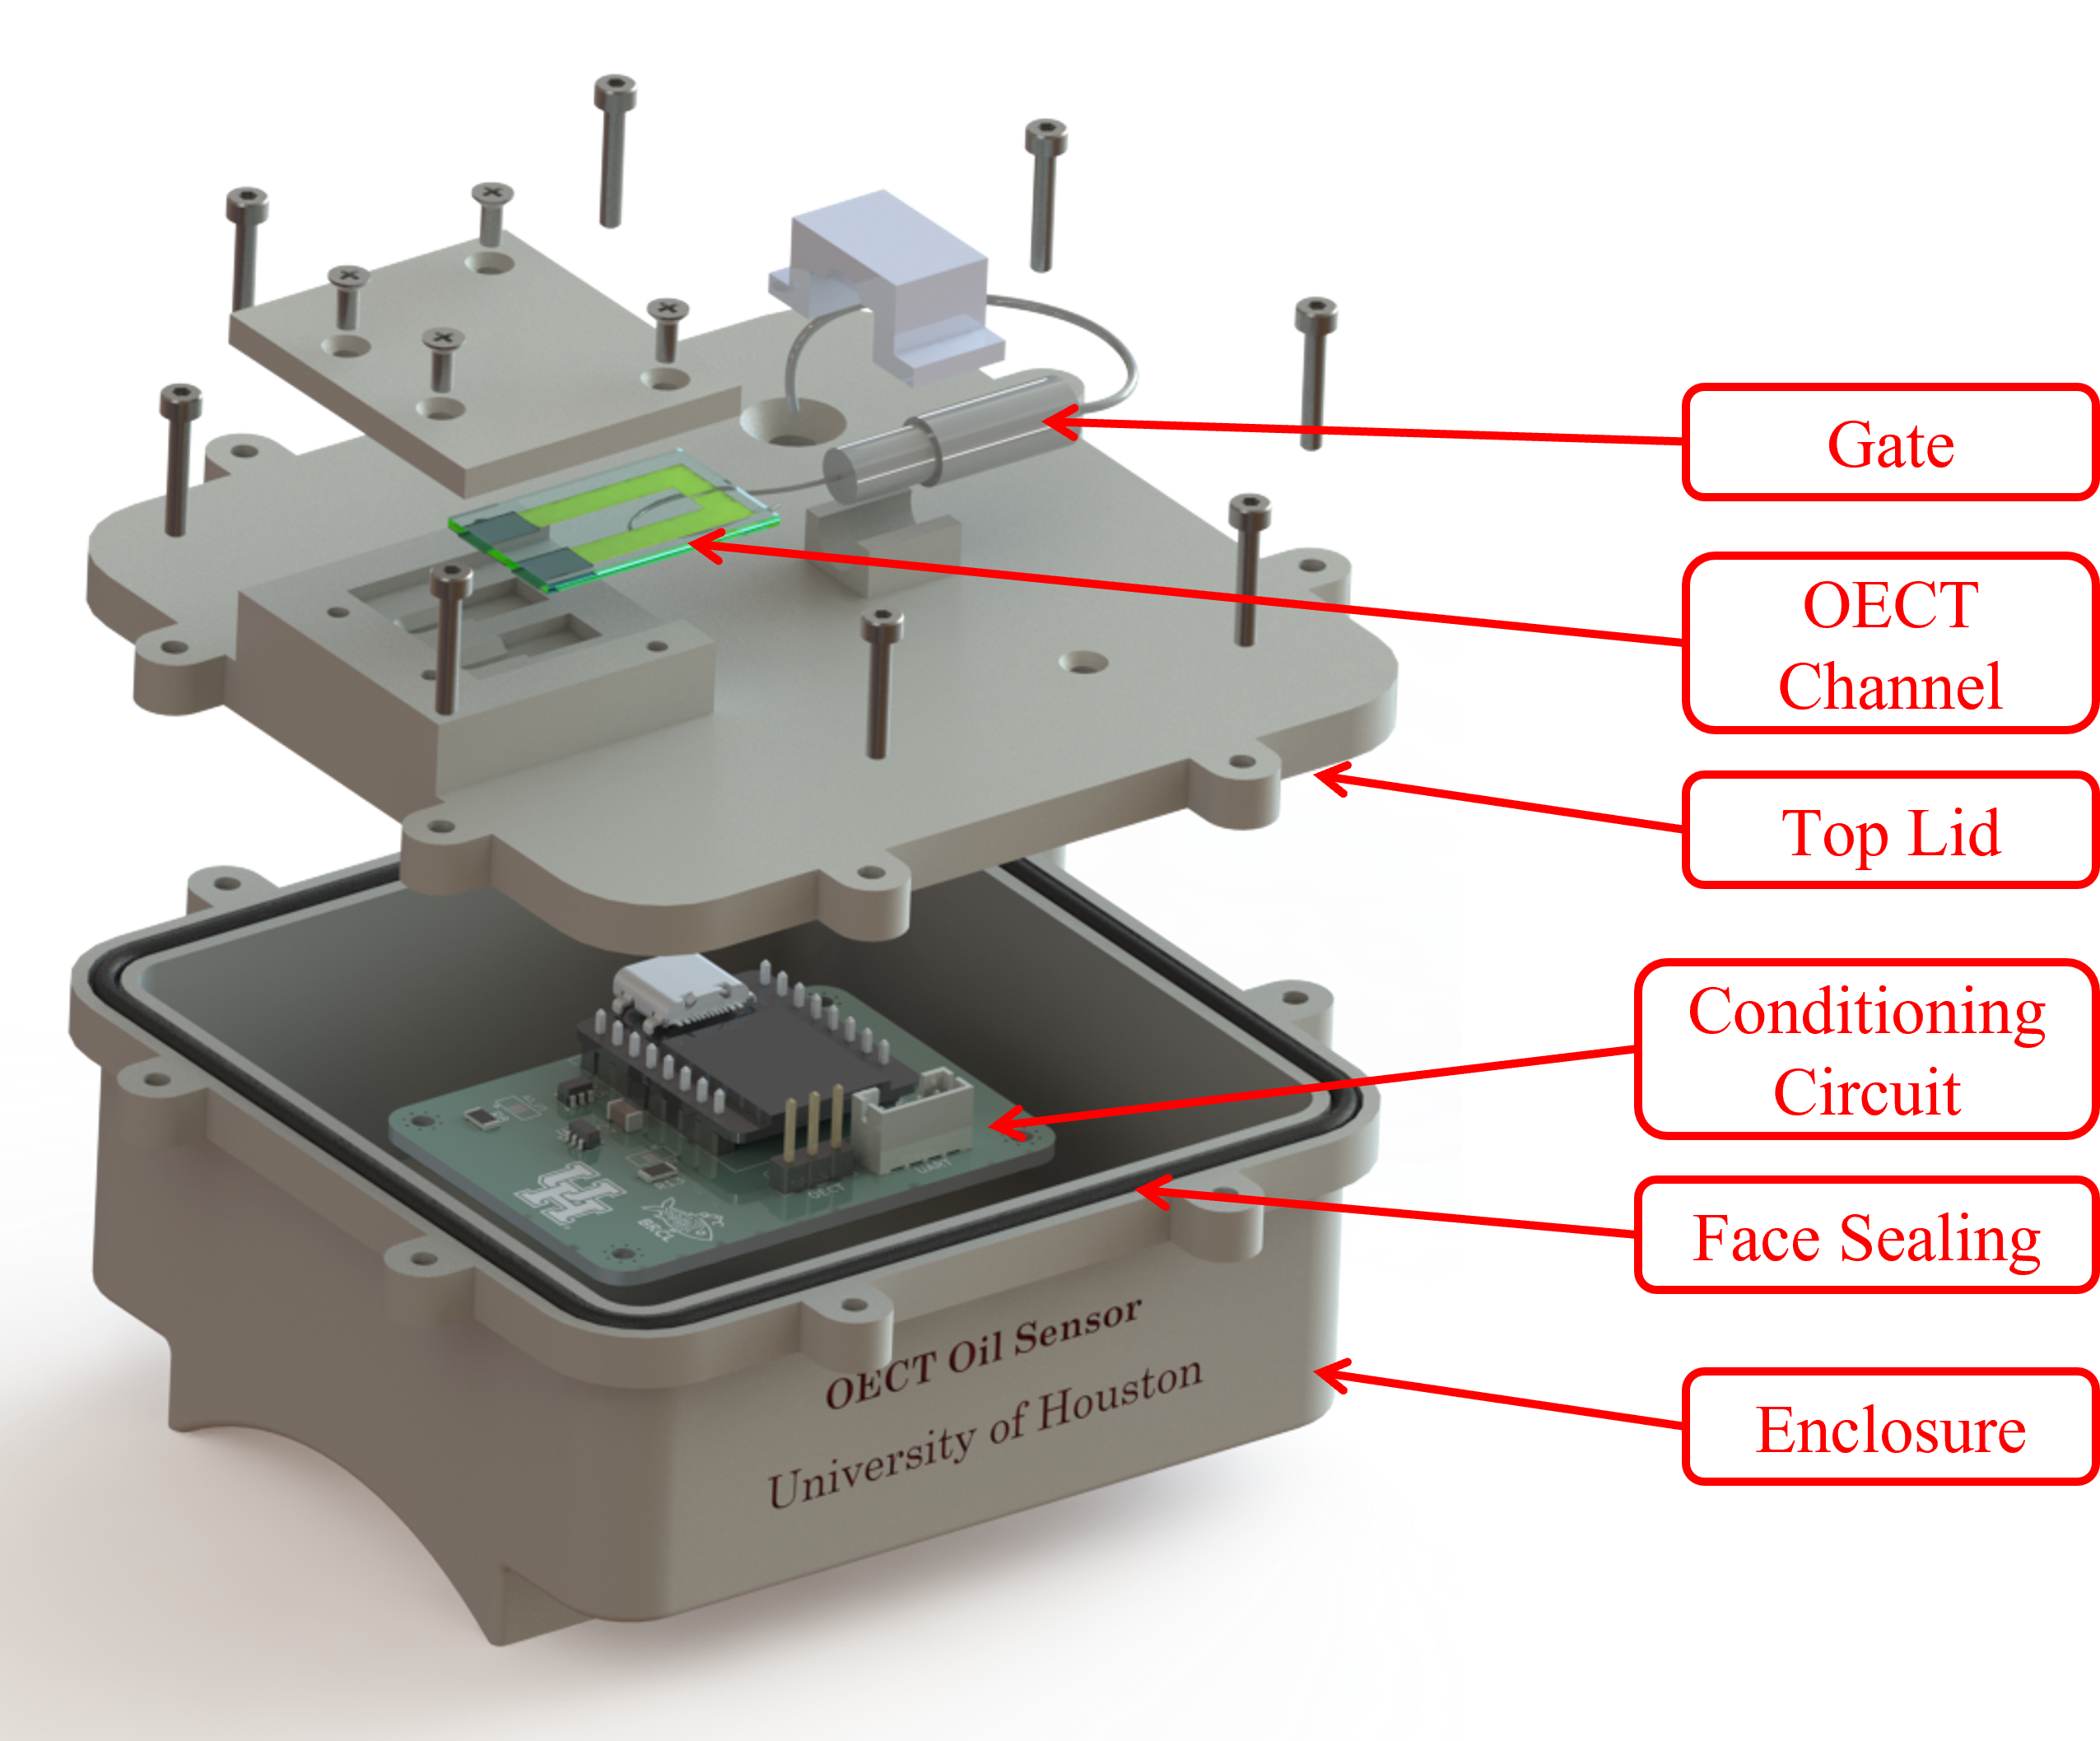
\includegraphics[width=0.7\textwidth]{figures/oect-enclosure-exploded.png}
    \caption{Enclosure for the OECT sensor and circuit}
    \label{fig:OECT-enclosure}
\end{figure}

\subsubsection{Water Tank Testing Setup}
For the proof-of-concept evaluation of the OECT sensor integrated into the AquaNavigator robotic fish, experiments are carried out in a water tank. The tank is sufficiently large to reproduce realistic oil leakage behavior and absorption. 
The tank was sufficiently large to allow oil leakage testing at the prototype scale. However, it still represents a partially controlled proof-of-concept environment rather than a coastal environment with open water. Although the experiments were not conducted in open coastal water, the testing environment was not completely idealized or static. The water tank included  water motion through a circulation system, and the robotic fish propulsion generated local hydrodynamic disturbance around the sensing region during operation. In addition, visible suspended particles and accumulated impurities were present in the testing environment, as shown in the experimental images and video. These conditions provided a moderate level of environmental disturbance while preserving sufficient control to isolate the integration of the OECT sensor, signal-conditioning circuit, and robotic fish platform. However, strong wave action, sediment resuspension, sand, mud, and floating debris were not independently controlled in the present study.
Its dimensions are 10 m in length, 5 m in width, and 1.5 m in depth. It is filled with fresh water, and a black oil pipeline is laid along the bottom. The pipeline is connected to a pump that circulates oil through the line. The oil flow is kept constant and regulated by a valve. A small hole is introduced at a specific location along the pipeline to enable oil to escape. This configuration creates a controlled simulation of an oil leak, in which the OECT sensor can be employed to detect the escaping oil.

The OECT sensor is subsequently integrated into the AquaNavigator robotic fish, which is programmed to swim along the pipeline. The signal conditioning circuit of the OECT sensor is equipped with a Serial UART interface, enabling communication with the AquaNavigator’s main control board. However, for experimental evaluation and to enable real-time visualization and logging of sensor data, the OECT sensor is interfaced with a host computer via the UART connection. The host computer runs the same MATLAB script that was used during laboratory testing.

\subsection{Lab results of OECT Characterization}
Fig. \ref{fig:oect-multi-solution-test} (Multi-solution test) presents the response time of the OECT in different liquid environments, including water, soda, seawater, and various oils. A triangular voltage waveform is applied to the gate as the input, and the resulting current response also follows a triangular pattern, revealing distinct electrical characteristics for each solution. Overall, the aqueous (non-oil) samples exhibit high conductivity within the OECT channel due to their ionic content, whereas the oil samples show markedly lower current levels, below 0.2 mA. This reduced current reflects the low conductivity in the OECT channel and signifies the presence of oil molecules. The periodic variations observable in all samples demonstrate the relationship between the input signal and the output current, which can be interpreted as hysteresis.

Fig. \ref{fig:oect-response-distribution} (response distribution) employs a box plot to compare current intensities across the different liquid samples, clearly highlighting the current decrease when the OECT is exposed to oil-based solutions. Consistent with the previous figure, the current response remains stable in non-oil samples, while contact with oil leads to a pronounced current reduction. Laboratory results confirm that the OECT provides an effective sensing strategy to determine the presence of oil molecules in liquid samples, and that triangular excitation is a practical approach to obtaining sensing results comparable to those from cyclic voltammetry.
\begin{figure}
    \centering
    
\includegraphics[width=0.75\textwidth]{figures/multi-solution-test.svg.png}
    \caption{The time response of the OECT sensor to the triangle excitation signal in different liquid samples.}
    \label{fig:oect-multi-solution-test}
\end{figure}
\begin{figure}
    \centering
    
\includegraphics[width=0.65\textwidth]{figures/response-distribution.png}
    \caption{The current distribution of the OECT sensor in various liquid samples shown as box plots.}
    \label{fig:oect-response-distribution}
\end{figure}

The OECT was characterized using an experimental setup in which the same water intended for use in a research pool for robot testing was employed and compared against seawater. Fig. \ref{fig:oect-response-oil-on-channel} presents the sensor’s response to the square wave generated by the circuit configuration shown in Fig. \ref{fig:CircuitBirdsEye}. The initial experiments were conducted with the sensor immersed in pool water and were repeated three times. The purple plots in Fig. \ref{fig:oect-response-oil-on-channel} correspond to the sensor response obtained in this phase. These three plots indicate that the sensor exhibits good repeatability in its response.

Subsequently, the experiment was carried out again using seawater collected from Galveston Beach in Houston. It was performed three times, and the blue curves shown in Fig. \ref{fig:oect-response-oil-on-channel} were obtained. These three curves are again very similar to one another, indicating that the sensor also exhibits good repeatability in its response to a square-wave signal in seawater. The sensor current in seawater is more than double that observed in pool water, which can be attributed to the higher salt content of seawater. This confirms that the sensor can clearly distinguish differences in the conductivity of the surrounding medium.

In the third step, a single drop of crude oil ($10\mu L$) was introduced directly into the OECT channel and the device was then immersed in seawater; this procedure was also carried out three times. In all three trials at this stage, the sensor’s response to gate excitation was nearly zero, indicating that the device no longer operated as a transistor once crude oil was injected directly into its channel. This result demonstrates that the sensor can clearly show the presence of crude oil by not responding to the gate voltage.

Injecting crude oil into the OECT channel prior to immersion in water is insufficient, as it does not accurately replicate the real conditions in which the robotic fish is intended to detect oil leakage in seawater. Therefore, in a separate experiment, two distinct quantities of crude oil were introduced into seawater, and the resulting sensor responses were recorded and compared with those obtained in pure seawater and in pool water. Fig. \ref{fig:oect-response-oily-water} presents the sensor response waveforms to the square-wave signal applied to the gate for the two crude-oil concentrations. Each experiment was conducted three times, and the consistency of the results confirms the repeatability of the procedure. A comparison of the plots for the two oil concentrations shows that the conductivity decreases as the crude oil concentration increases. These findings demonstrate that the sensor can not only detect the presence of crude oil but, when properly characterized, can also discriminate between different oil concentrations.
\begin{figure}
    \centering
    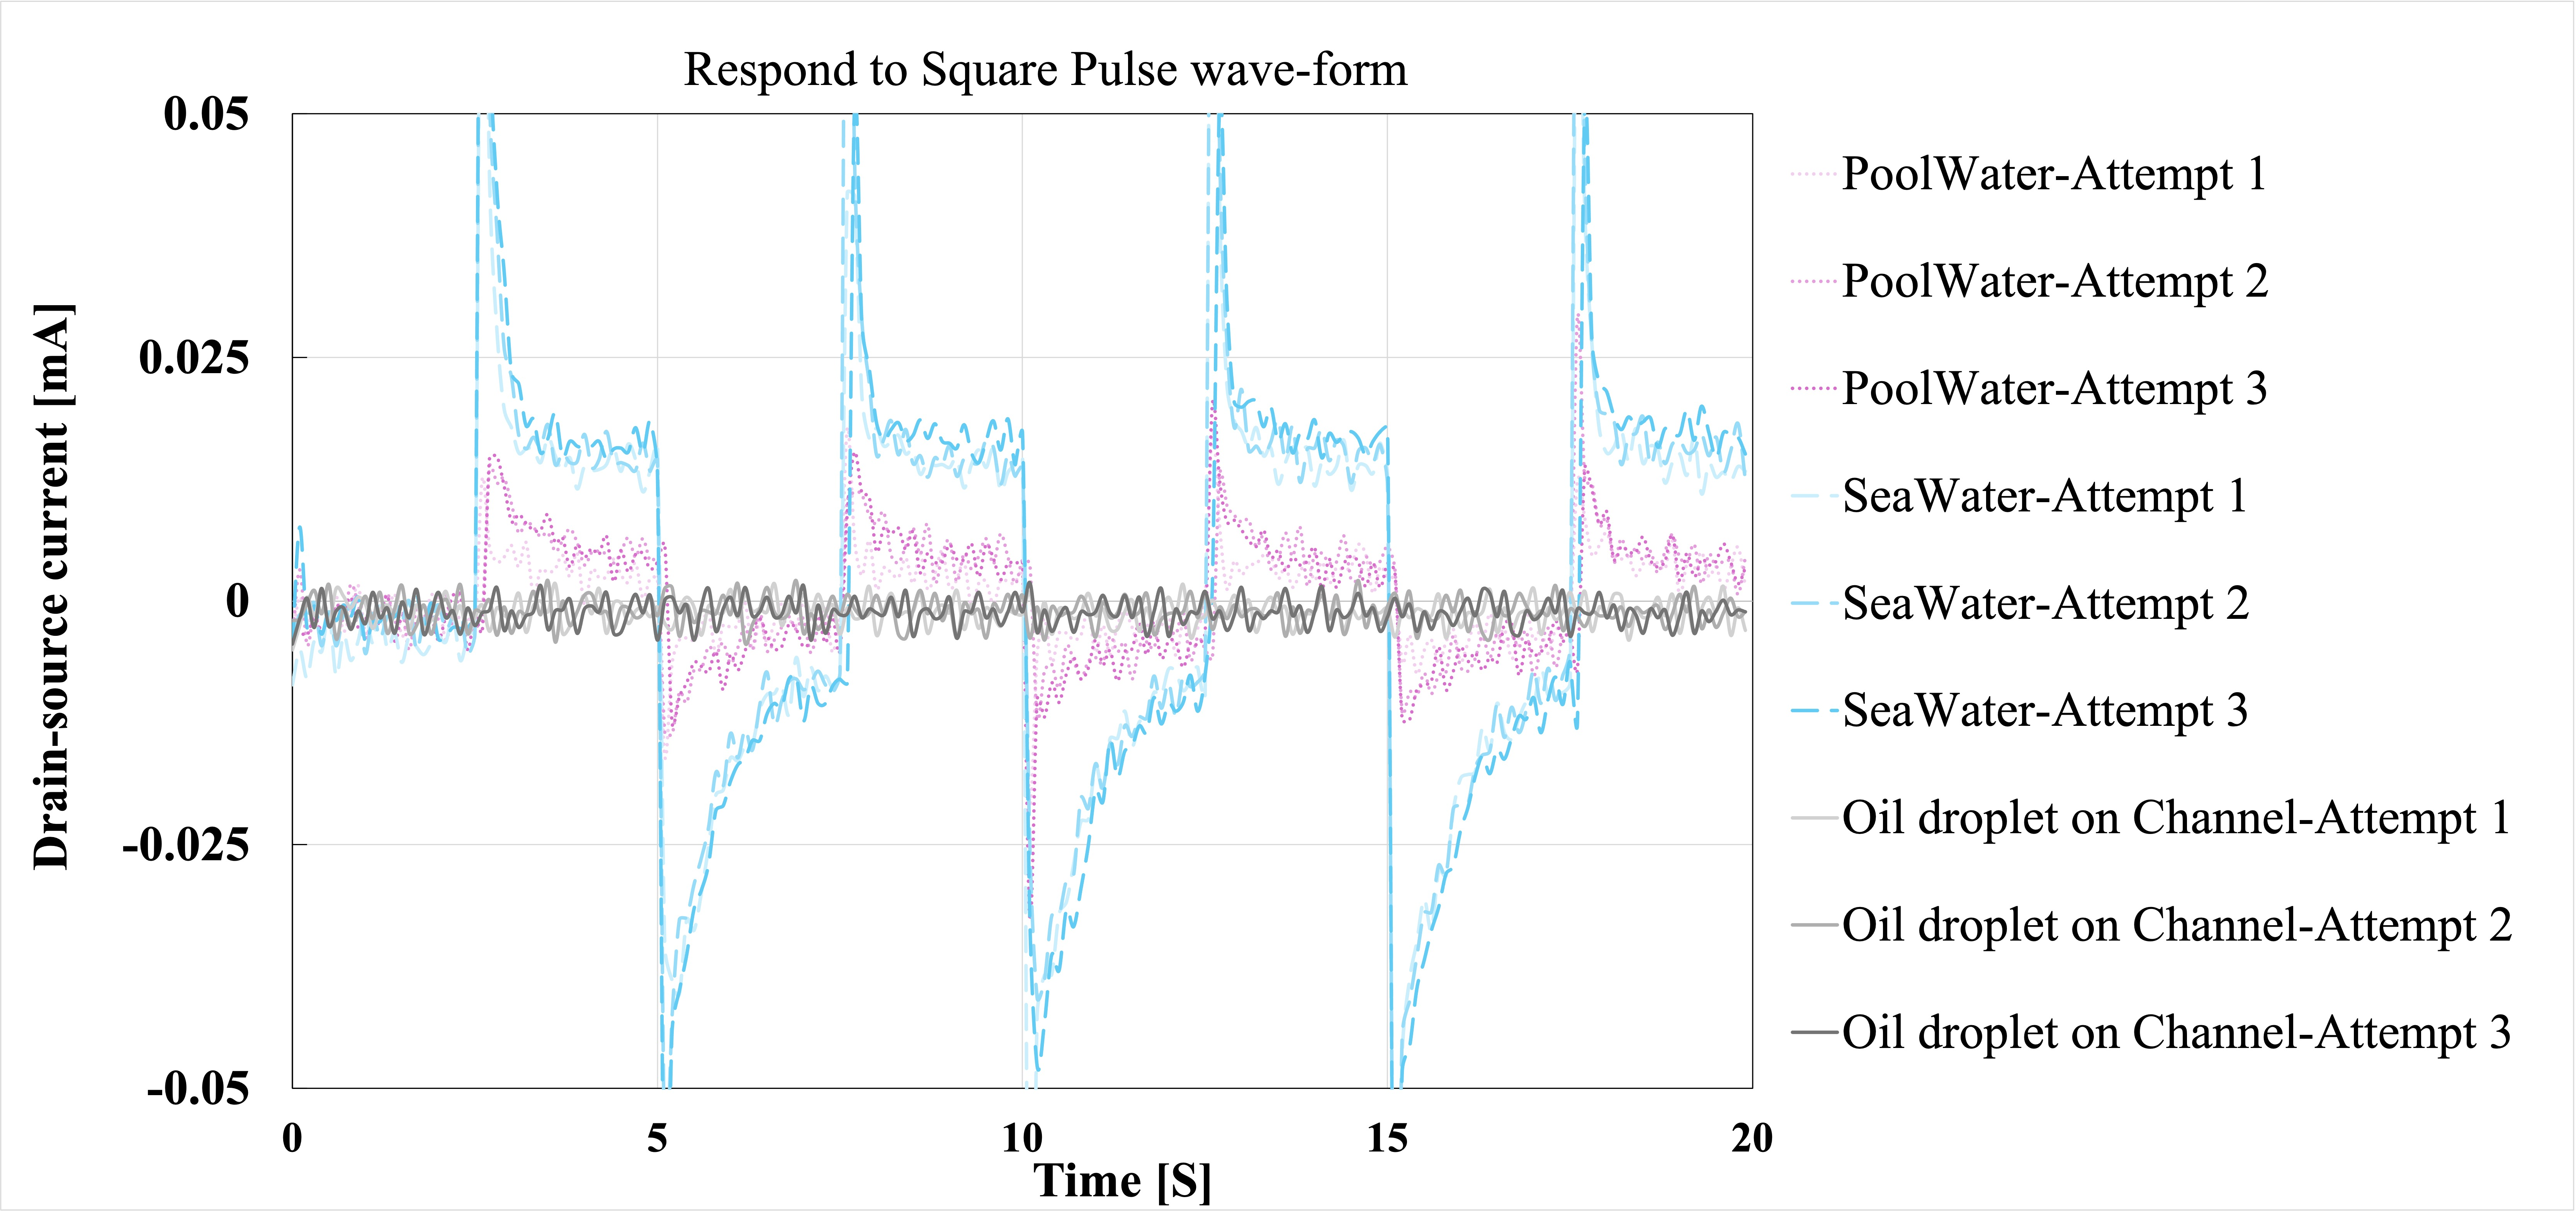
\includegraphics[width=0.65\textwidth]{figures/CircuitTestOilonChannel.jpg}
    \caption{The response of the sensor while it is tested with the circuit setup for current measurement instead of source measurement unit and oil droplet is injected directly on the channel of the OECT before being immersed into water.}
    \label{fig:oect-response-oil-on-channel}
\end{figure}
\begin{figure}
    \centering
    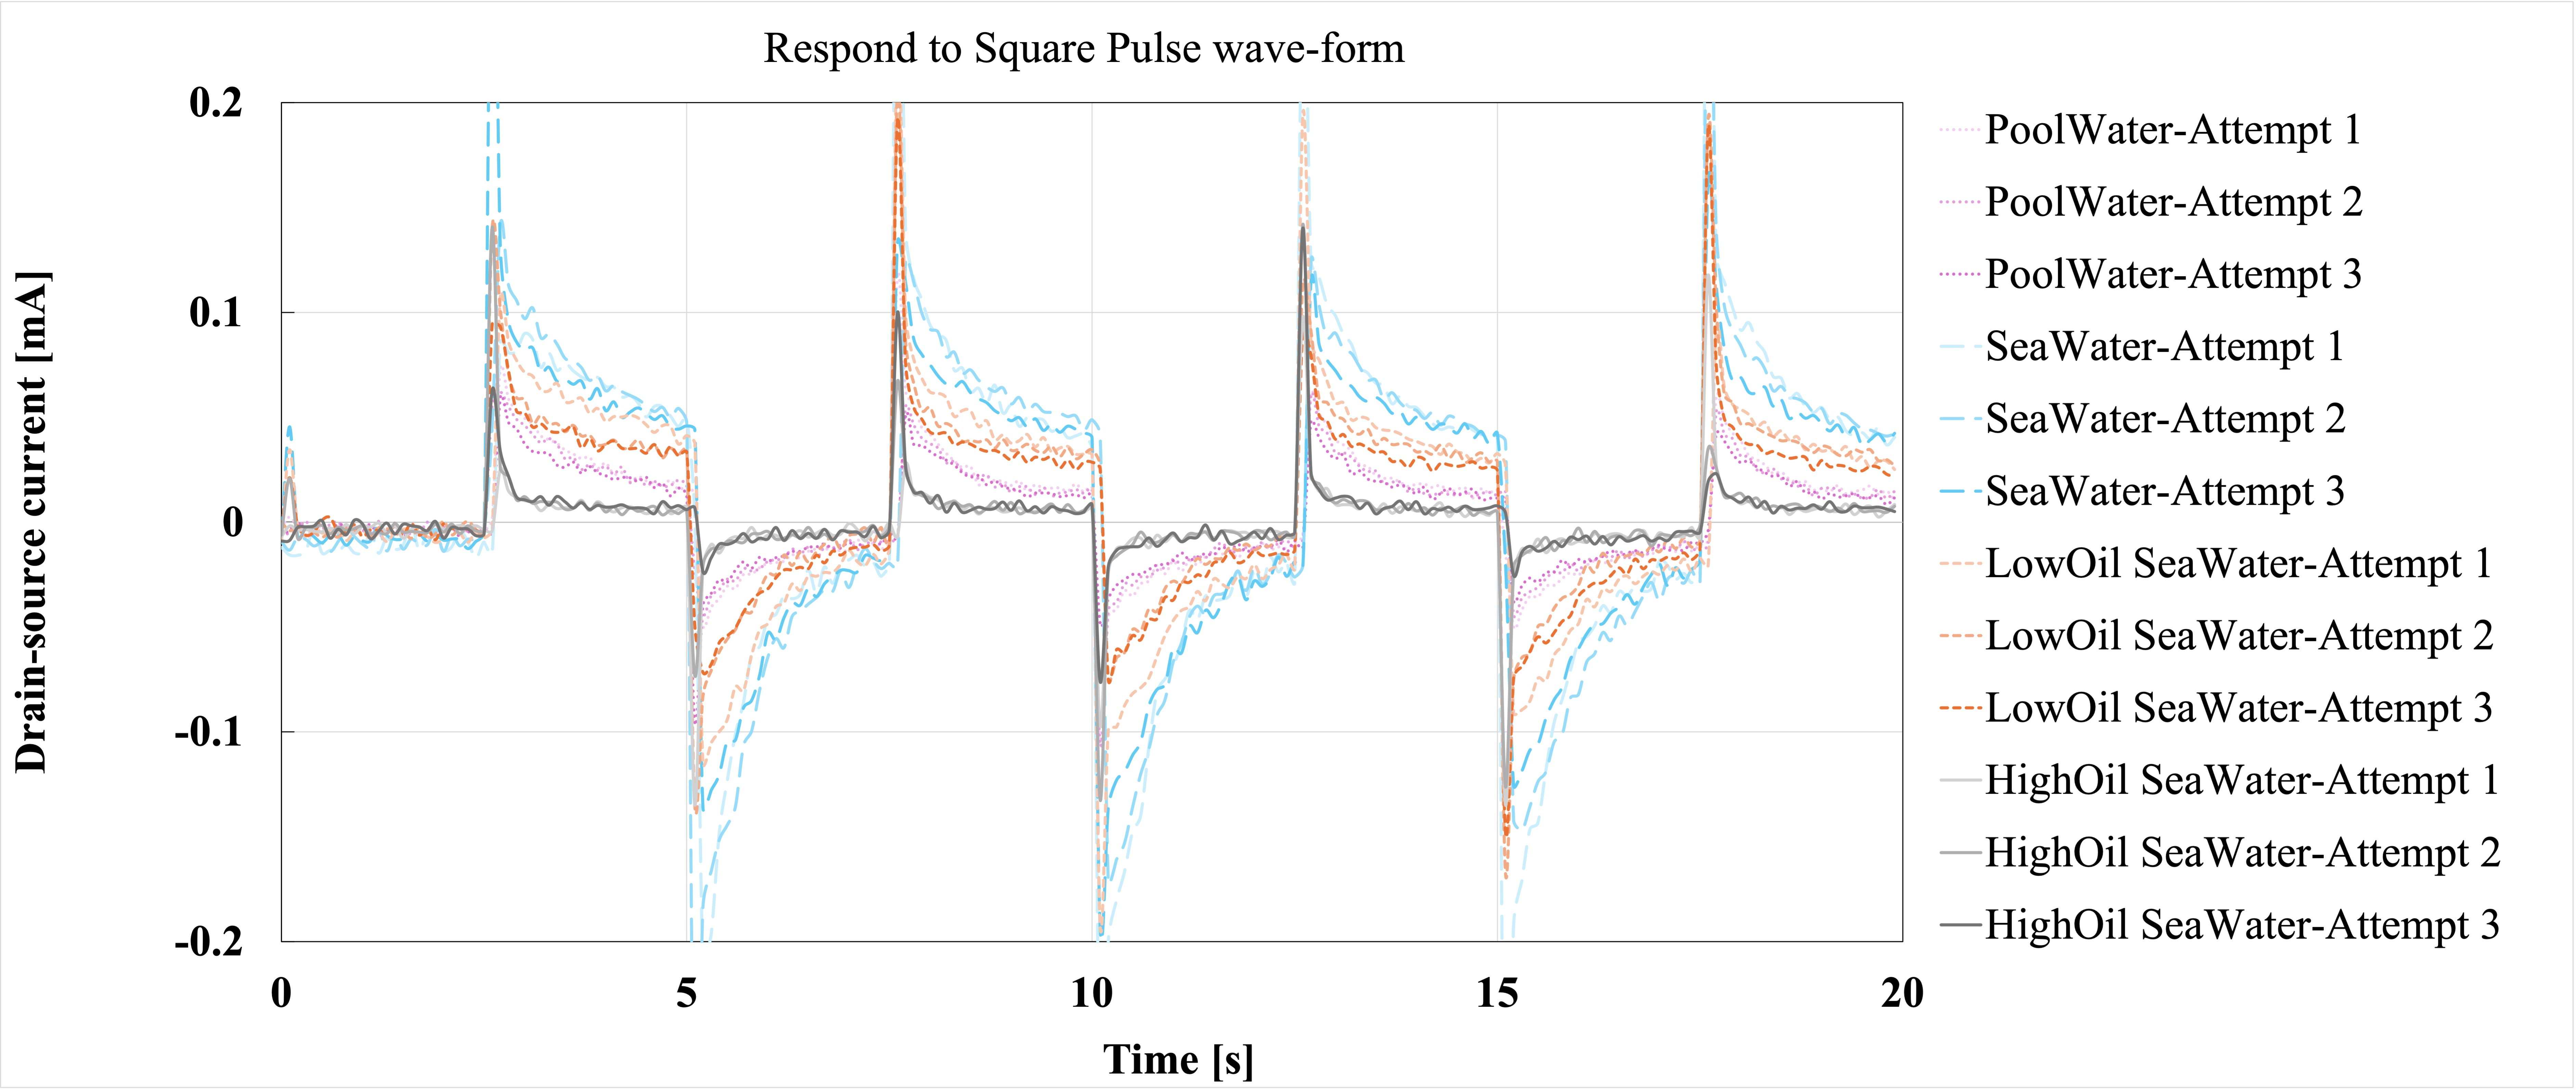
\includegraphics[width=0.65\textwidth]{figures/CircuitTestOilyWater.jpg}
    \caption{The response of the sensor while it is tested with the circuit setup for current measurement instead of source measurement unit while oil is added to water with concentrations of 4,and 8 g/L.}
    \label{fig:oect-response-oily-water}
\end{figure}

\subsection{Water Tank results of OECT with robotic fish}
The AquaNavigator, an intelligent underactuated robotic fish, functions as the platform for the OECT sensor, enabling flexible and real-time monitoring of oil spills in aquatic settings. To assess the sensor’s performance under realistic operating conditions, the robotic fish is programmed to autonomously follow a pipeline in a water tank using an image-based visual servoing strategy. The onboard camera streams video to a host computer, where the pipeline is detected and control commands are computed and sent to the fish’s main control board to drive the motors. As detailed in our earlier work \cite{masood2025visual}, two principal parameters are employed to quantify tracking performance: the heading error angle $\psi_e$, defined as the angle between the robot’s current heading and the desired heading toward the projected point on the pipeline, and the pixel distance $y$ between the tip of the heading vector and the target point on the pipeline. Beyond these image-derived indicators, tracking precision is further examined by measuring the fish’s angular deviation from the intended heading vector and its lateral offset from the pipeline, as depicted in Fig. \ref{fig:robotic-fish-tracking}.

\begin{figure}[htp!]
    \centering
    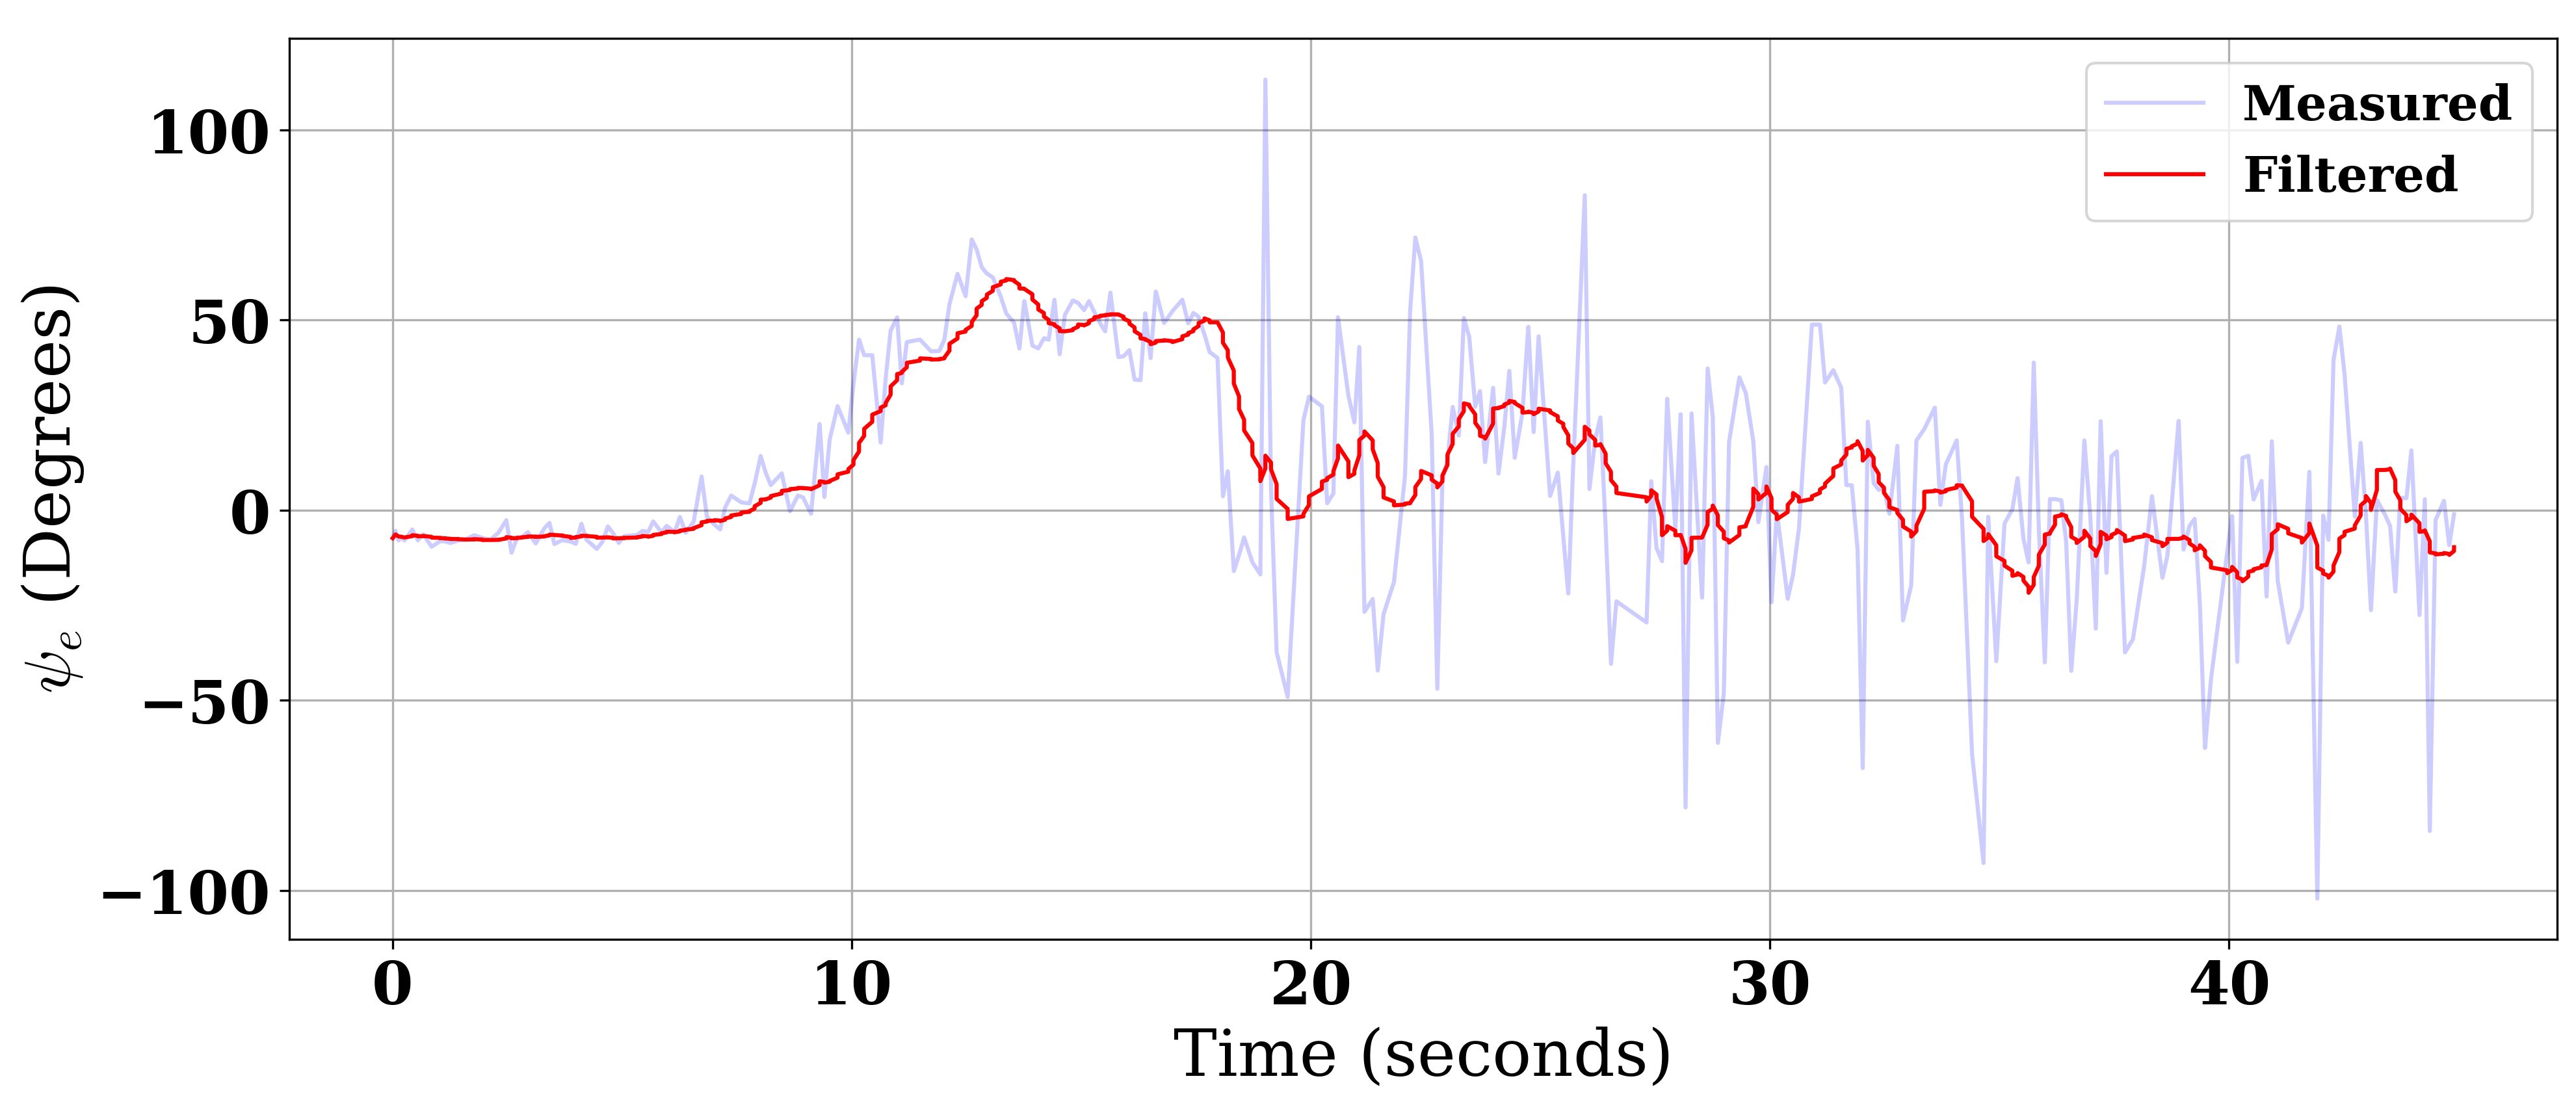
\includegraphics[width=0.75\textwidth]{figures/pipeline_tracking_plot_20250813_154401_psie.png}
    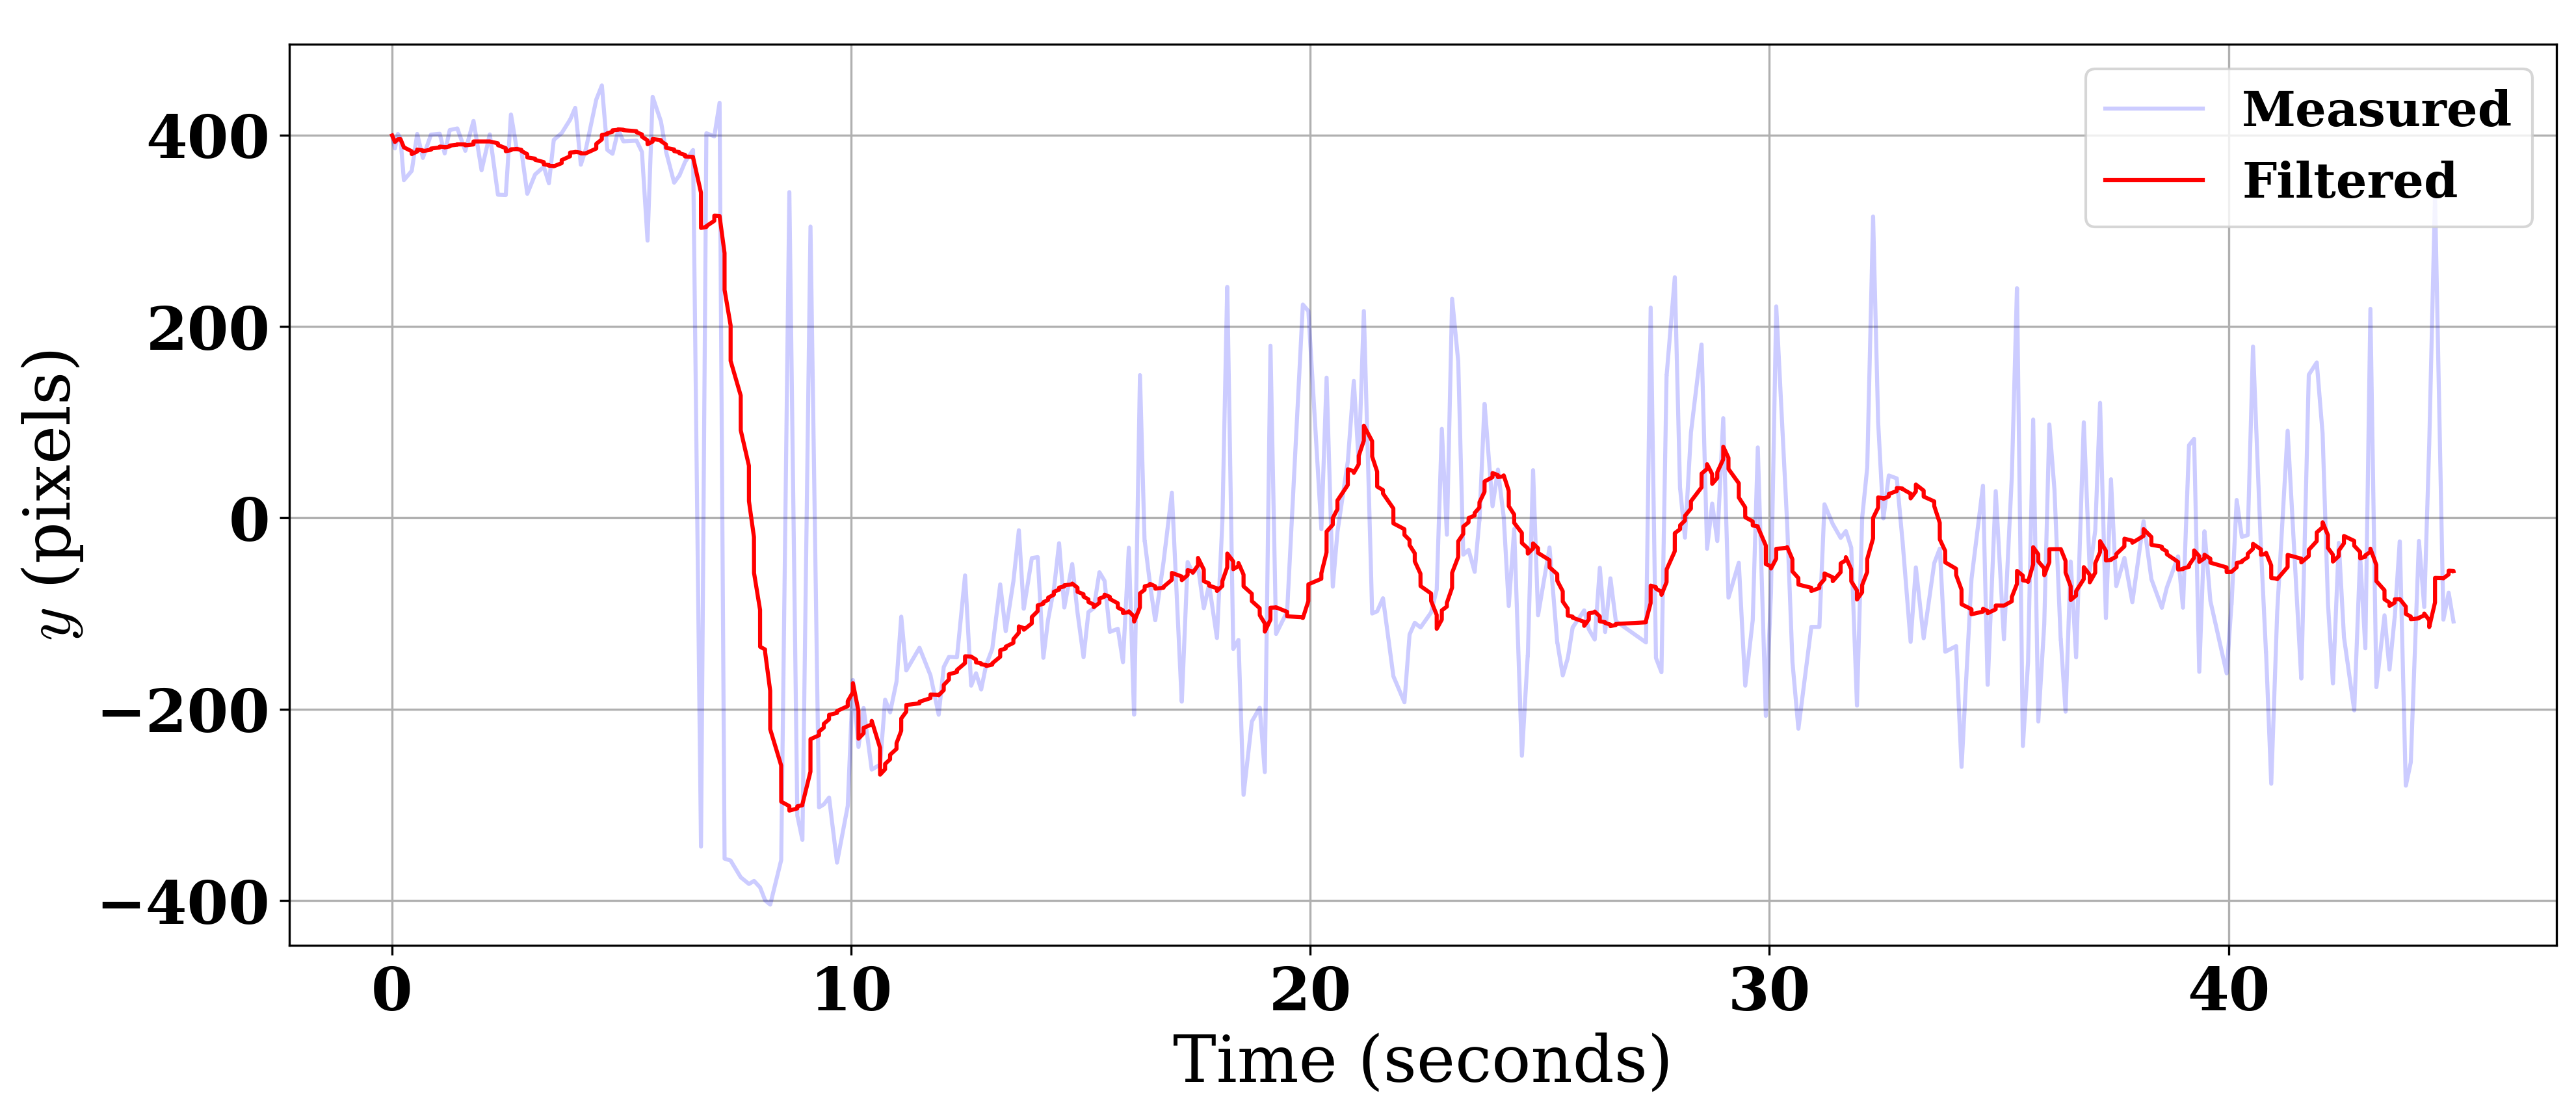
\includegraphics[width=0.75\textwidth]{figures/pipeline_tracking_plot_20250813_154401_y.png}
    \caption{Robotic fish tracking performance along the pipeline.}
    \label{fig:robotic-fish-tracking}
\end{figure}
\begin{figure}[htp!]
    \centering
    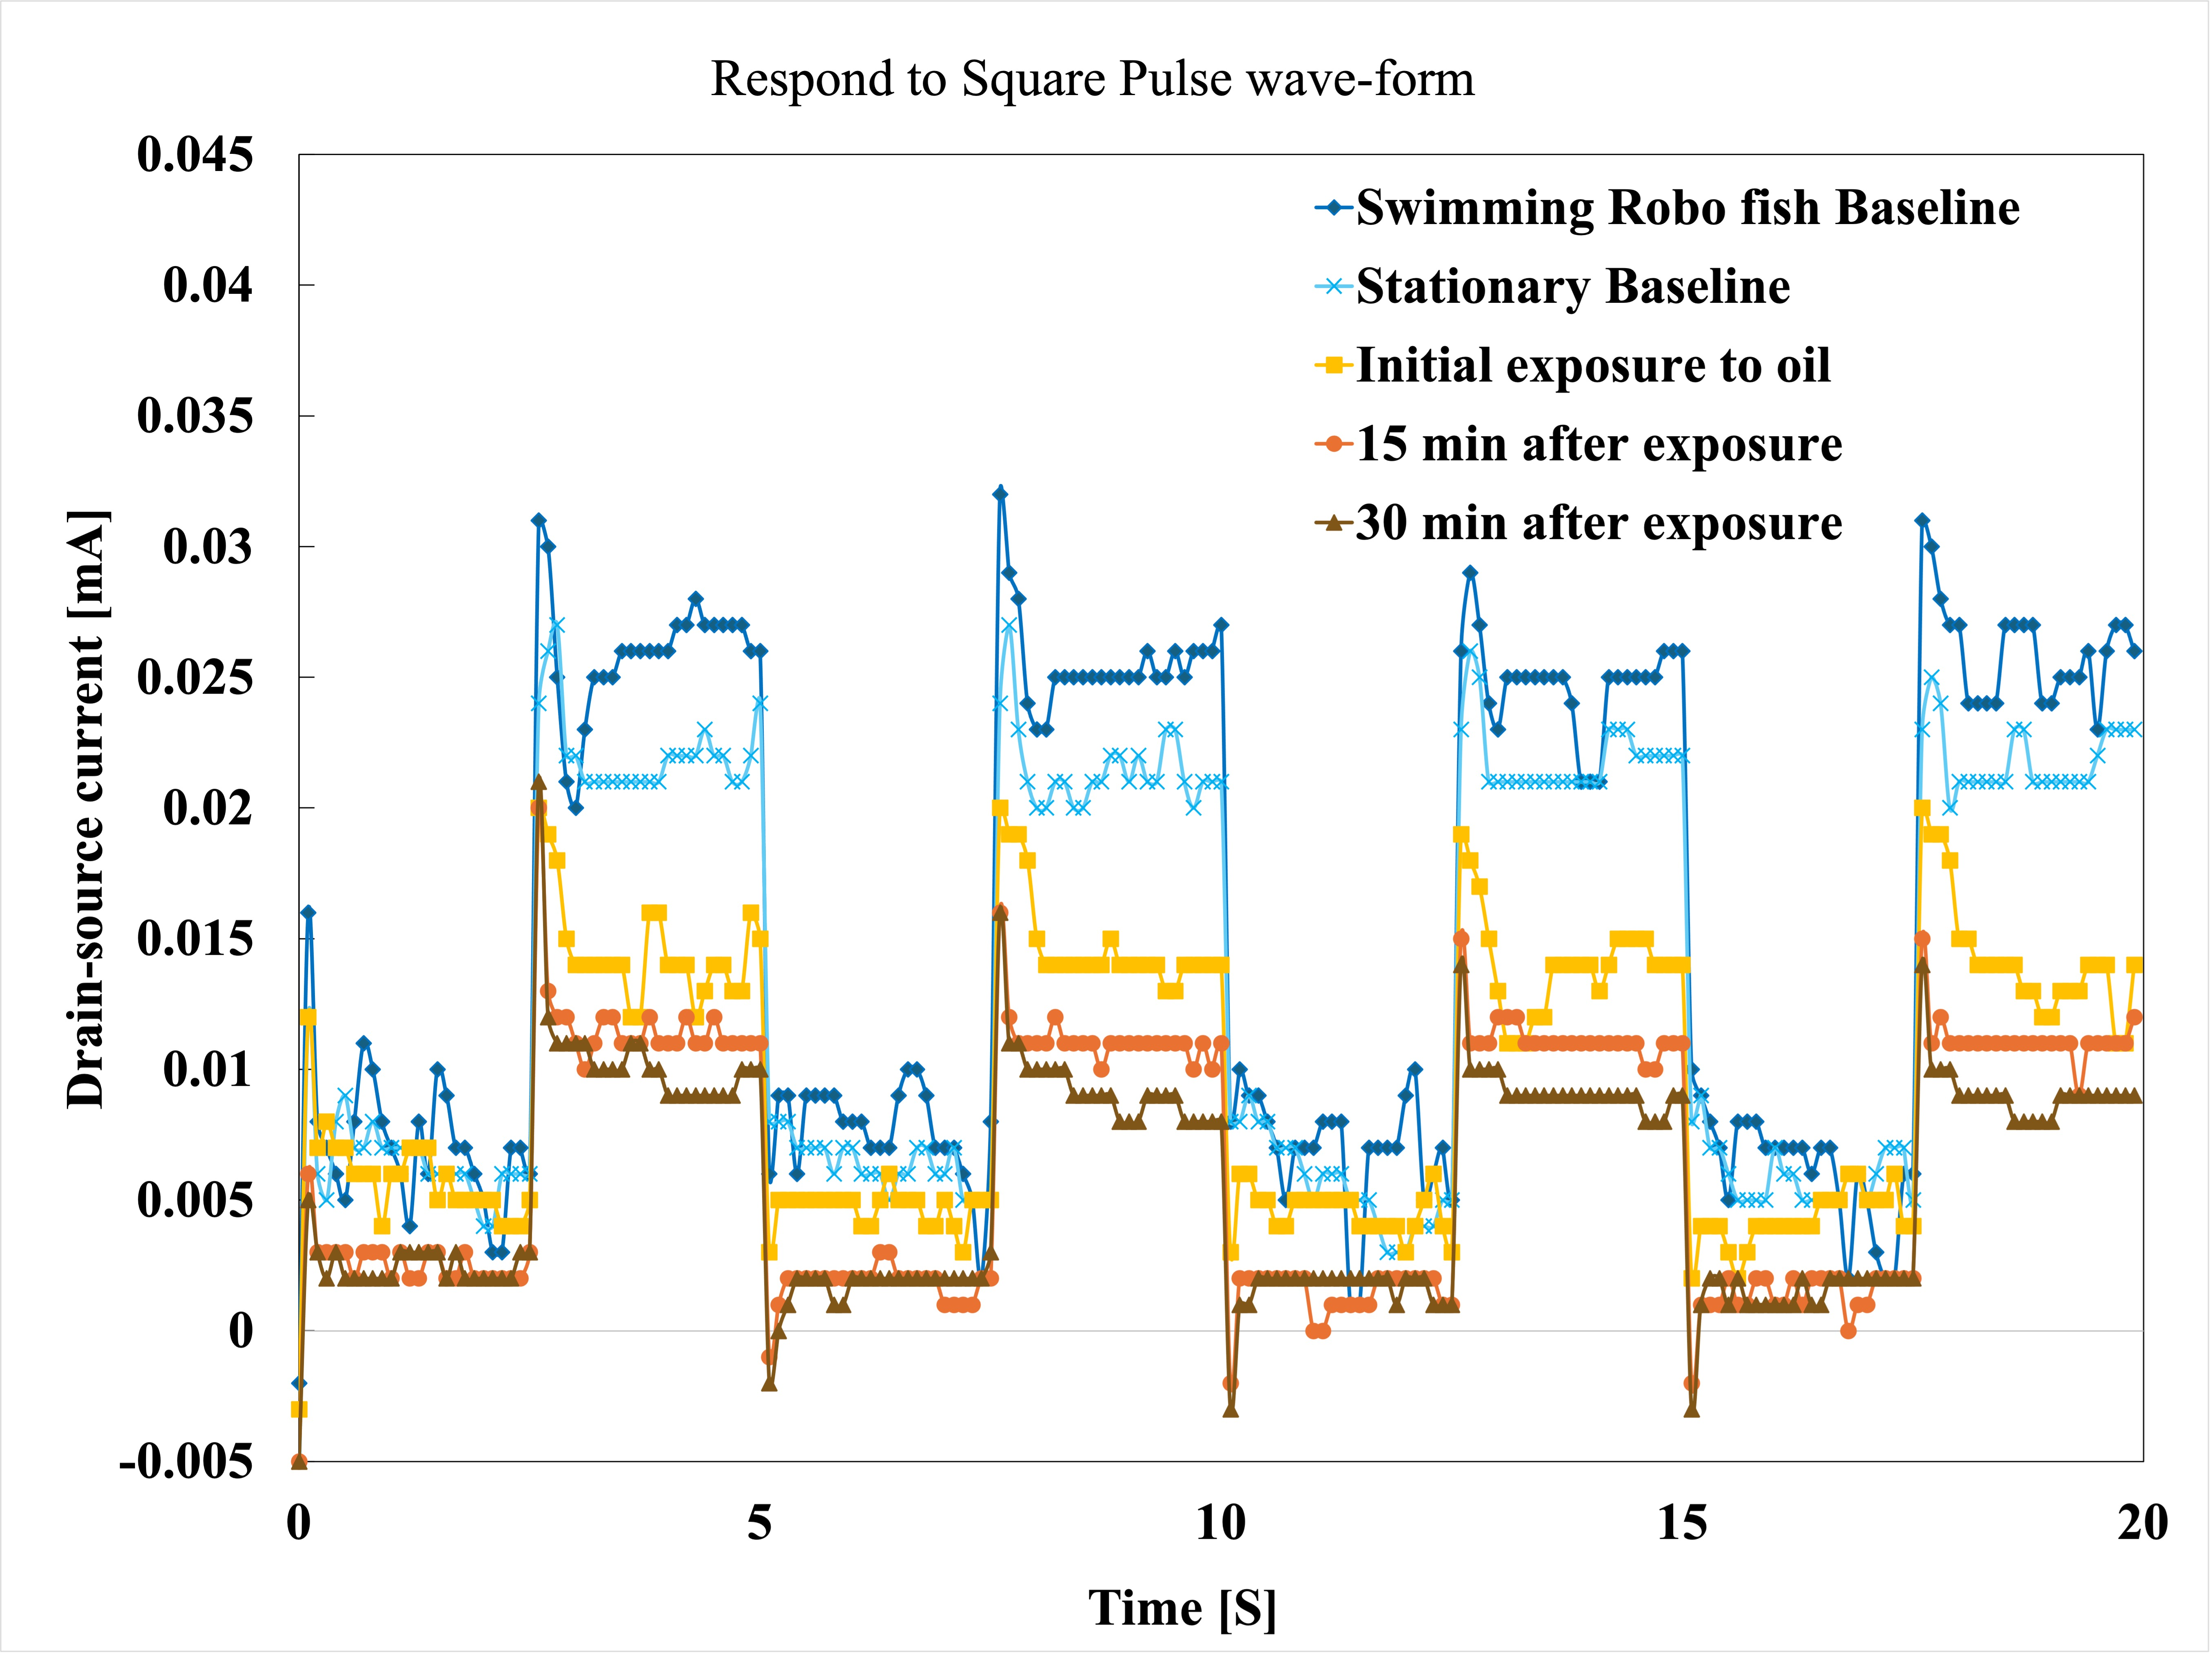
\includegraphics[width=0.75\textwidth]{figures/AnalyzedTechBridge updated.jpg}
    \caption{Response without oil leakage compared with three different exposure levels of the sensor to contaminated water.}
    \label{fig:allMeasruementsPool}
\end{figure}

For the integration system tests, the sensor was installed on the AquaNavigator and evaluated in a pool while the robotic fish followed a pipeline. A photograph of the robotic fish during this experimental stage is provided in Fig. \ref{fig:robofishInPool}. The sensor’s response to a square-wave input was first measured with the robotic fish held stationary and with no oil present in the pool, providing the baseline for the experiment. The sensor response was then measured again as the robotic fish traversed the pipeline, still in oil-free conditions. This procedure was used to determine whether the motion of the robotic fish affected the sensor output. Both measurements were repeated three times to verify the repeatability of the results. The sensor responses without oil, for the stationary and moving robotic fish, are shown as the light and dark blue curves, respectively, in Fig. \ref{fig:allMeasruementsPool}.

After establishing the baseline and identifying the influence of movement, an oil leak was introduced at a defined position along the pipeline to evaluate whether the robotic fish could detect the leak while passing that point. A constant oil flow rate of 5 ml/min was supplied to the rupture site via a peristaltic dosing pump. The yellow curve in Fig. \ref{fig:allMeasruementsPool} represents the sensor signal in the contaminated region. These results demonstrate that the sensor reliably detected the oil leak as the robotic fish traversed the polluted area. Following the initial detection of contamination, the robotic fish remained within that region to pinpoint the exact location of the leak. It should be noted that the sensor showed an approximately 60-second delay in the change in amplitude after the robotic fish entered the contaminated zone, which is attributed to the oil absorption time within the OECT channel. Because oil was leaking continuously near the rupture point, the oil concentration in the contaminated zone increased over time. Consequently, by keeping the robotic fish in the highly polluted area, the OECT channel is expected to absorb more oil, producing a more pronounced decrease in the measured current amplitude. The experiment was repeated twice: once 15 minutes after the initial detection of contamination and again after 30 minutes. The orange and brown curves in Fig. \ref{fig:allMeasruementsPool} depict the sensor responses after 15 and 30 minutes of exposure to the contaminated area, respectively. This figure illustrates the progressive reduction in the OECT response with increasing exposure time to the oil leak. 
\\
The current water tank experiments support the feasibility of detecting an oil leak with the integrated OECT–robotic fish platform under controlled but moderately disturbed conditions. However, the tests do not fully replicate shallow coastal environments, where waves, currents, sediment resuspension, mud, sand, biological fouling, and floating debris can affect system performance. These factors may influence detection by altering the contact time between oil and the OECT channel. They can also partially block the sensing surface, alter the local conductivity of the surrounding water, disturb the robot’s attitude, or degrade camera-based pipeline tracking. Accordingly, the present results should be interpreted as proof-of-concept validation of the integrated sensing platform rather than complete field validation. Future work should include systematic robustness tests under controlled wave and current conditions, varying turbidity and sediment levels, debris exposure, and ultimately open-water coastal tests.

\section{Conclusion}
This paper presented a practically implementable approach to locating the source of oil spills using a bio-inspired robotic fish platform. An OECT sensor was engineered to detect crude oil in aqueous media, including seawater, with high sensitivity and stability. A dedicated signal conditioning circuit for the sensor was developed to support real-time monitoring and classification of oil contamination. The AquaNavigator robotic fish platform was configured to carry the OECT sensor, providing mobility and adaptability for a range of underwater applications. Laboratory evaluations of the OECT sensor confirmed its capability to detect oil concentrations as low as 10 µg, while the signal conditioning circuit enabled efficient data collection. Experiments conducted in a water tank verified the effectiveness of both the OECT sensor and the AquaNavigator platform in identifying oil spills, thereby demonstrating the practicality of using this type of sensor for locating oil spill sources in aquatic environments. The proposed system shows promise for environmental monitoring, underwater exploration, and search and rescue missions. Future research will examine how the sensor’s mounting position influences detection performance and will assess the system in more realistic subsea scenarios, where oil is released at depth and must travel upward before forming a detectable slick at the surface.
Future research will examine how the sensor’s mounting position can affect detection performance and will further assess the system in more realistic coastal and subsea scenarios, including disturbances created by wave and current. It will also include sediment or mud resuspension, suspended sand and particles, floating debris, and oil released at depth that must travel upward before forming a detectable slick at the surface.
% use section* for acknowledgment
\ack{This research is supported by the Texas Commission on Environmental Quality through an award to the Subsea Systems Institute. This project was funded [in part] with federal funding from the Department of Treasury through the State of Texas under the 2012 Resources and Ecosystems Sustainability, Tourist Opportunities, and Revived Economies of the Gulf Coast States Act (RESTORE Act). The content, statements, findings, opinions, conclusions, and recommendations are those of the author(s) and do not necessarily reflect the views of the State of Texas or the Treasury.}
% Can use something like this to put references on a page
% by themselves when using endfloat and the captionsoff option.
% \ifCLASSOPTIONcaptionsoff
%   \newpage
% \fi
% \bibliographystyle{IEEEtran}
% \section*{References}
\bibliographystyle{iopart-num}
\bibliography{bibliography}

%\vspace{11pt}
\end{document}
